\documentclass[10pt,]{scrartcl}
\usepackage{lmodern}
\usepackage{amssymb,amsmath}
\usepackage{ifxetex,ifluatex}
\usepackage{fixltx2e} % provides \textsubscript
\ifnum 0\ifxetex 1\fi\ifluatex 1\fi=0 % if pdftex
  \usepackage[T1]{fontenc}
  \usepackage[utf8]{inputenc}
\else % if luatex or xelatex
  \ifxetex
    \usepackage{mathspec}
  \else
    \usepackage{fontspec}
  \fi
  \defaultfontfeatures{Ligatures=TeX,Scale=MatchLowercase}
\fi
% use upquote if available, for straight quotes in verbatim environments
\IfFileExists{upquote.sty}{\usepackage{upquote}}{}
% use microtype if available
\IfFileExists{microtype.sty}{%
\usepackage[]{microtype}
\UseMicrotypeSet[protrusion]{basicmath} % disable protrusion for tt fonts
}{}
\PassOptionsToPackage{hyphens}{url} % url is loaded by hyperref
\usepackage[unicode=true]{hyperref}
\PassOptionsToPackage{usenames,dvipsnames}{color} % color is loaded by hyperref
\hypersetup{
            pdftitle={Measuring coherence with Bayesian Networks},
            colorlinks=true,
            linkcolor=blue,
            citecolor=blue,
            urlcolor=blue,
            breaklinks=true}
\urlstyle{same}  % don't use monospace font for urls
\usepackage{graphicx,grffile}
\makeatletter
\def\maxwidth{\ifdim\Gin@nat@width>\linewidth\linewidth\else\Gin@nat@width\fi}
\def\maxheight{\ifdim\Gin@nat@height>\textheight\textheight\else\Gin@nat@height\fi}
\makeatother
% Scale images if necessary, so that they will not overflow the page
% margins by default, and it is still possible to overwrite the defaults
% using explicit options in \includegraphics[width, height, ...]{}
\setkeys{Gin}{width=\maxwidth,height=\maxheight,keepaspectratio}
\IfFileExists{parskip.sty}{%
\usepackage{parskip}
}{% else
\setlength{\parindent}{0pt}
\setlength{\parskip}{6pt plus 2pt minus 1pt}
}
\setlength{\emergencystretch}{3em}  % prevent overfull lines
\providecommand{\tightlist}{%
  \setlength{\itemsep}{0pt}\setlength{\parskip}{0pt}}
\setcounter{secnumdepth}{5}
% Redefines (sub)paragraphs to behave more like sections
\ifx\paragraph\undefined\else
\let\oldparagraph\paragraph
\renewcommand{\paragraph}[1]{\oldparagraph{#1}\mbox{}}
\fi
\ifx\subparagraph\undefined\else
\let\oldsubparagraph\subparagraph
\renewcommand{\subparagraph}[1]{\oldsubparagraph{#1}\mbox{}}
\fi

% set default figure placement to htbp
\makeatletter
\def\fps@figure{htbp}
\makeatother

%\documentclass{article}

\usepackage[table]{xcolor
}


% %packages
 \usepackage{booktabs}
 \usepackage[sort&compress]{natbib}
\usepackage{graphicx}
\usepackage{longtable}
\usepackage{ragged2e}
\usepackage{etex}
%\usepackage{yfonts}
\usepackage{marvosym}
\usepackage[notextcomp]{kpfonts}
\usepackage{nicefrac}
\newcommand*{\QED}{\hfill \footnotesize {\sc Q.e.d.}}

\usepackage[textsize=footnotesize]{todonotes}
%\linespread{1.5}



\setlength{\parindent}{10pt}
\setlength{\parskip}{1pt}


%language
%\usepackage{times}
\usepackage{mathptmx}
\usepackage{t1enc}
%\usepackage[utf8x]{inputenc}
%\usepackage[polish]{babel}
%\usepackage{polski}

\usepackage{subcaption}


%AMS
\usepackage{amsfonts}
\usepackage{amssymb}
\usepackage{amsthm}
\usepackage{amsmath}

%\usepackage{geometry}
 %\geometry{a4paper,left=35mm,top=20mm,}

%abbreviations
\newcommand{\ra}{\rangle}
\newcommand{\la}{\langle}
\newcommand{\n}{\neg}
\newcommand{\et}{\wedge}
\newcommand{\jt}{\rightarrow}
\newcommand{\ko}[1]{\forall  #1\,}
\newcommand{\ro}{\leftrightarrow}
\newcommand{\exi}[1]{\exists\, {_{#1}}}
\newcommand{\pr}{\mathsf{P}}
\newcommand{\odds}{\mathsf{Odds}}
\newcommand{\ind}{\mathsf{Ind}}
\newcommand{\nf}[2]{\nicefrac{#1\,}{#2}}
\newcommand{\R}[1]{\texttt{#1}}

\newtheorem{q}{\color{blue}Question}



\newcommand{\s}[1]{\mbox{\textsf{#1}}}



\newtheorem*{reply*}{Reply}
\usepackage{enumitem}
\newcommand{\question}[1]{\begin{enumerate}[resume,leftmargin=0cm,labelsep=0cm,align=left]
\item #1
\end{enumerate}}

\usepackage{float}

% \setbeamertemplate{blocks}[rounded][shadow=true]
% \setbeamertemplate{itemize items}[ball]
% \AtBeginPart{}
% \AtBeginSection{}
% \AtBeginSubsection{}
% \AtBeginSubsubsection{}
% \setlength{\emergencystretch}{0em}
% \setlength{\parskip}{0pt}

\title{Measuring coherence with Bayesian Networks}
\author{}
\date{\vspace{-2.5em}}

\begin{document}
\maketitle

\begin{abstract} \textbf{Abstract.} The notion of coherence is often used in many philosophical, especially epistemological, discussions (for instance, in discussions  about the  truth-conduciveness of coherence). An explication of the key notion involved seems desirable.  We introduce the most prominent coherence measures and a number of counterexamples put forward against them.  Then, we point out some common problems that underlie these counterexamples. These observations lead  us to a new measure of coherence. Our measure  diverges from the known candidates in three important respects: (1) It is not a function of a probabilistic measure and a set of propositions alone, because it is also sensitive to the selection and direction of arrows in a Bayesian network representing an agent's credal state. (2) Unlike in the case of quite a few coherence measures, it is not obtained by taking a mean of some list of intermediate values (such as confirmation levels between subsets of a narration). It  is sensitive also to the variance and the minimal values of the intermediate values. (3) The intermediate values used are not confirmation levels, but rather expected and weighted confirmation levels. We apply our measure to the existing counterexamples and compare its performance to the performance of the other measures. It does a  better job. 


\vspace{3mm}

\footnotesize

\noindent \textbf{Technical remark.} The whole work has been made possible by all those who contributed to the development of \textsf{\textbf{R}} language, and Marco Scutari, the author of \textsf{\textbf{bnlearn}} package, who was kind enough to extend his package with additional features upon our requests. The use of these tools here is essential, because we used the environment to write Bayesian Networks (BNs) for all the counterexamples, all coherence functions as applicable to BNs (including ours), and automated  performance analysis and BN visualisation, which otherwise wouldn't  be manageable. Our code with a guide can be made available to the reviewer upon request, and will be available open access if the paper is published.



\end{abstract}

\section{Motivations \& introduction}

The notion of coherence is often used in many philosophical, especially
epistemological, discussions (for instance, in discussions about the
truth-conduciveness of coherence). An explication of the key notion
involved seems desirable.

There is also a more practical reason to develop a better understanding
of the notion: a plausible measure of coherence could be used to better
evaluate the quality of some stories or narrations. For example in the
legal context we would like to be able to assess the quality of a
testimony in the court of law. Focusing only on the probability of a
story is to some extent problematic, because from such a perspective,
more detailed stories are penalized --- they contain more propositions,
so they (usually) have lower probabilities. A plausible coherence
measure could be used to asses an important aspect of a narration which
so far seems to escape probabilistic analysis.

When we talk about the coherence of a set of propositions or about the
coherence of a story, we seem to refer to how well their individual
pieces fit together. How are we to understand and apply this notion
systematically, though?

As with beliefs, we can use both a binary and a graded notion of
coherence. The binary notion is not very exciting: a set is incoherent
just in case it is logically
inconsistent.\footnote{There is a related notion in the neighborhood where an agent's  degrees of beliefs are coherent just in case it they are probabilistic. We will not use this notion in this paper.}
Intuitively, graded coherence should be a generalization of this
requirement: logically incoherent sets should have minimal (or at least
negative) level of graded coherence. Or, at least, lower coherence than
consistent ones. What other requirements should a coherence measure
satisfy and how should it be explicated formally, if we want to massage
this notion into a more general framework of probabilistic epistemology?
Defining a measure of graded coherence in probabilistic terms turned out
to be quite a challenge, which resulted in heaps of literature.

Also, in reasarch unconnected to and seemingly unaware of the
philosophical discussion, in the context of Bayesian networks developed
for stories and narrations in legal contexts (C. Vlek et al., 2013, C.
Vlek et al. (2014), C. S. Vlek et al. (2015), C. Vlek (2016), Fenton et
al. (2013), Fenton et al. (2013)), an approach to coherence has been
developed by Vlek. The proposal is to capture the coherence of the story
by introducing a single narration root node which becomes an ancestor
node to all the other nodes such that the conditional probability of
each dependent node given that the state of this root is 1 (that is, the
corresponding proposition is assumed to be true), is also 1. This is
defended by observing that in such a network previously independent
nodes become dependent without any principled reason. This is true, but
we don't think this is desirable: one shouldn't introduce probabilistic
dependencies by fiat in a model. Moreover, Vlek then identifies
coherence of a model with the prior probability of the narration node,
and we specifically want to capture the idea that coherence is distinct
from probability. For this reason, we think an account of coherence for
such practical applications is still missing.

We first introduce the main existing coherence measures. Then we
describe a lengthy list of counterexamples to these measures. A general
discussion of certain common features and issues we observed follows,
which leads us to the description of our own coherence measure.

Our measure diverges from the known candidates in three important
respects: (1) It is not a function of a probabilistic measure and a set
of propositions alone, because it is also sensitive to the selection and
direction of arrows in a Bayesian Network representing an agent's credal
state. (2) Unlike in the case of quite a few coherence measures, it is
not obtained by taking a mean of some list of intermediate values (such
as confirmation levels between subsets of a narration). It is sensitive
also to the variance and the minimal values of the intermediate values.
(3) The intermediate values used are not confirmation levels, but rather
expected and weighted confirmation levels (read on for details).
Finally, we apply our measure to the existing counterexamples and
compare its performance to the performance of the other measures.
Spoiler alert: it does a better job.

\section{Measures}

Let's take a look at different approaches to measuring coherence. One
thing to keep in mind is that different measures use different scales
and have different neutral points, if any (the idea is: the coherence of
probabilistically independent propositions should be neither positive
nor negative).

\subsection{Deviation from independence -- Shogenji}

The first measure we present was developed by Tomoji Shogenji (1999, p.
340) and is often called \textit{deviation from independence}. This
measure is defined as the ratio between the probability of the
conjunction of all claims, and the probability that the conjunction
would get if all its conjuncts were probabilistically independent.

\begin{align}
    \tag{Shogenji}
    \label{coh:Shogenji}
    C_s(A_1,\dots,A_n)=\frac{P(A_1 \& \dots \& A_n)}{P(A_1)\times\dots\times P(A_n)}
\end{align}

\noindent \textbf{scale:} {[}0, \(\infty\){]}

\noindent  \textbf{neutral point:} 1

\noindent This measure was later generalized by Meijs \& Douven (2007).
According to this approach, \eqref{coh:Shogenji} is applied not only to
the whole set of propositions, but to each non-empty non-singleton
subset of the set, and the final value is defined as the average of all
sub-values thus obtained.

\subsection{Relative overlap -- Olsson \& Glass}

The second approach, a \textit{relative overlap} measure, comes from
Olsson (2001) and Glass (2002). This measure is defined as the ratio
between the intersection of all propositions and their union. It was
later generalized in a way analogous to the one used in the
generalization of the Shogenji's measure.

\begin{align}
    \tag{Olsson}
    \label{coh:Olsson}
    C_o(A_1,\dots,A_n)=\frac{P(A_1 \& \dots \& A_n)}{P(A_1 \vee \dots \vee A_n)}
\end{align}

\noindent \textbf{scale:} {[}0, 1{]}

\noindent \textbf{neutral point:} NO

\subsection{Average mutual support}

Finally, the most recent approach --- a class of measures called
\textit{average mutual support}. The general recipe for such a measure
is this.

\begin{itemize}
\item
  Given that \(S\) is a set whose coherence is to be measured, let \(P\)
  indicate the set of all ordered pairs of non-empty, disjoint subsets
  of \(S\).
\item
  First, define a confirmation measure for the confirmation of a hypothesis \(H\) by evidence  \(E\): \(Conf(H,E)\).
\item
  For each pair \(\langle X, Y \rangle \in P\), calculate
  \(Conf(\bigwedge X, \bigwedge Y)\), where $\bigwedge X$ ($\bigwedge Y$) is the conjunction of all the elements of $X$ ($Y$).
\item
  Take the mean of all the results.
\end{itemize}\begin{align*}
    \mathcal{C}(P) & =
mean\left(\left\{Conf(\bigwedge X_i, \bigwedge Y_i) | \langle X_i, Y_i \rangle \in P\right\} \right)
\end{align*}

\noindent Depending on the choice of a confirmation measure, we achieve
different measures of coherence.

\subsubsection{Fitelson}

Fitelson (2003a, 2003b) uses the following confirmation function:

\begin{align*}
    F(H,E) = \begin{cases}
    1 & E\models H, E\not \models \bot \\
    -1 & E \models \neg H\\
    \frac{P(E|H)-P(E|\neg H)}{P(E|H)+P(E|\neg H)} & \mbox{o/w}
    \end{cases}
\end{align*}

\begin{align}
\tag{Fitelson}  
    \mathcal{C}_{F}(P) & =
mean\left(\left\{F(\bigwedge X_i, \bigwedge Y_i) | \langle X_i, Y_i\rangle \in P\right\} \right)
\end{align}

\noindent For instance, Fitelson's coherence for two propositions boils
down to this:

\begin{align}    
    \tag{Fitelson pairs}  
    \mathcal{C}_{F}(X,Y) &= \frac{F(X,Y)+F(Y,X)}{2}
    \label{coh:Fitelson}
\end{align}

\noindent \textbf{scale:} {[}-1, 1{]}

\noindent \textbf{neutral point:} 0

\subsubsection{Douven and Meij's}

Another coherence measure of this type has been introduced by Douven \&
Meijs (2007).

They use the \textit{difference} confirmation measure:

\begin{align*}
    D(H,E) = P(H|E) - P(H)
\end{align*}

The resulting definition of coherence is:

\begin{align}
\tag{DM}  
    \mathcal{C}_{DM}(P) & =
mean\left(\left\{D(\bigwedge X_i, \bigwedge Y_i) | \langle X_i, Y_i\rangle \in P\right\} \right)
\end{align}

For two propositions, the coherence measure boils down to:

\begin{align}
    \tag{DM pairs}
    \label{coh:DM}
    C_{DM}(X,Y)= \frac{P(X|Y) - P(X) + P(Y|X) - P(Y)}{2}
\end{align}

\noindent \textbf{scale:} {[}-1, 1{]}

\noindent \textbf{neutral point:} 0 (not explicit)

\subsubsection{Roche}

Yet another measure, due to Roche (2013, p. 69), starts with the
absolute confirmation measure:

\begin{align*}
    A(H,E) = \begin{cases}
    1 & E\models H, E\not \models \bot \\
    0 & E \models \neg H\\
    P(H|E) & \mbox{o/w} \\
    \end{cases}
\end{align*}

which results in the following coherence measure:

\begin{align}
\tag{Roche}  
    \mathcal{C}_{R}(P) & =
mean\left(\left\{A(\bigwedge X_i, \bigwedge Y_i) | \langle X_i, Y_i\rangle \in P\right\} \right) 
\end{align}

For two propositions, the measure gives the following:

\begin{align}
    \tag{Roche pairs}
    \label{coh:Roche}
     C_{R}(X,Y)= \frac{P(X|Y)+P(Y|X)}{2}
\end{align}

\noindent \textbf{scale:} {[}0, 1{]}

\noindent \textbf{neutral point:} 0.5

\section{Challenges}

One methodological approach to the discussion about measures of
coherence relies on the assumption that various explications proposed in
the literature can be criticized by pointing out thought experiments
which inspire coherence-related intuitions that disagree with a given
coherence measure. Of course, the idea that principled philosophical
accounts should be tested against thought experiments that are hopefully
easier to agree on than general philosophical claims themselves is
debatable. However, this paper does not aim to address this general
question. Instead, in line with the discussion, we take the challenges
posed by counterexamples seriously, and ask the following question: is
there a fairly sensible probabilistic explication of the notion of
coherence which is not undermined by the existing counterexamples? This
does not mean that we take these examples as some sort of ultimate
benchmark. Conceptual explication does have to start somewhere, and key
seemingly clear-cut cases against probabilistic explications of
coherence seem to be a decent candidate. If you care about the problem,
and are worried about the counterexamples, this paper aims to address
your concerns.

So here is a selection counterexamples put forward against various
probabilistic coherence measures in the literaturesudo . We attempted to
list those that were picked up in the discussion, a few where both we
didn't share the authors' intuitions and the examples were not picked up
in further discussion in the literature.\footnote{One example, involving
  Sarah and her pregnancy (Tomoji Shogenji, 2006), but it focused more
  on truth-conduciveness of coherence, which is beyond the scope of our
  paper. We also do not discuss a few other examples involving fossils
  and voltage (T. Shogenji, 2001; Mark Siebel, 2006). In some respects,
  they were quite similar to the dice and depth problems that we do
  discuss, and some of their variants simply did not inspire our
  agreement. For instance, Siebel thinks that for voltage levels
  \(\{V=1, V=2\}\) is more coherent than \(\{V=1, V=50\}\), while we
  think that both sets are maximally incoherent (there might be some
  claims in the vincinity that are not incoherent, say, focusing on
  results of separate measurements, but an example along these lines has
  not been properly formulated in the literature).}

\subsection{Penguins}

\textbf{The scenario.} A challenge discussed in (Bovens \& Hartmann,
2004, p. 50) and (Meijs \& Douven, 2007) consists of the following set
of propositions (instead of \emph{letters} or \emph{abbreviations},
we'll talk about \emph{nodes}, as these will be used later on in
Bayesian networks):

\begin{table}[H]
\centering
\begin{tabular}{ll}
\toprule
node & content\\
\midrule
\cellcolor{gray!6}{B} & \cellcolor{gray!6}{Tweety is a bird.}\\
G & Tweety is a grounded animal.\\
\cellcolor{gray!6}{P} & \cellcolor{gray!6}{Tweety is a penguin.}\\
\bottomrule
\end{tabular}
\end{table}

\noindent \textbf{Desiderata.} It seems that the set \{\s{B},\s{G}\},
which doesn't contain the information about Tweety being a penguin,
should be less coherent than the one that does contain this information:
\{\s{B},\s{G},\s{P}\}.

\vspace{2mm}

\begin{description}
    \item[(\s{BG}$<$\s{BGP})] \{\s{B},\s{G}\}  should be less coherent than \{\s{B},\s{G},\s{P}\}. 
\end{description}

\vspace{2mm}

Another intuition about this scenario (Schippers \& Koscholke, 2019) is
that when you consider a set which says that Tweety is both a bird and a
penguin: \{\s{B},\s{P}\}, adding proposition about not flying (\s{G})
shouldn't really increase the coherence of the set. It's a well-known
fact that penguins don't fly, and so one can deduce \s{G} from \s{P}.
Therefore by adding \s{G} explicitly to the set, one wouldn't gain any
new information -- so if a set expresses the same information, its
coherence shouldn't be different. As \s{G} is not a logical consequence
of \s{P}, it can be argued that \{\s{B},\s{P}\} and
\{\s{B},\s{P},\s{G}\} represent different information sets, and a slight
difference in their coherence is also acceptable.

\vspace{2mm}

\begin{description}
    \item[(\s{BP}$\approx$\s{BGP})]  \{\s{B},\s{P}\} should have similar coherence to \{\s{B},\s{P},\s{G}\}.  
\end{description}

\vspace{2mm}

\subsection{Dunnit}

\textbf{The scenario.} Another challenge, introduced by Merricks (1995)
goes as follows: Mr.~Dunnit is a suspect in the murder case. Detectives
first obtained the following body of evidence:

\begin{table}[H]
\centering
\begin{tabular}{l>{\raggedright\arraybackslash}p{25em}}
\toprule
node & content\\
\midrule
\cellcolor{gray!6}{I} & \cellcolor{gray!6}{Witnesses claim to have seen Dunnit do it (incriminating testimony).}\\
M & Dunnit had a motive for the murder.\\
\cellcolor{gray!6}{W} & \cellcolor{gray!6}{A credible witness claims to have seen Dunnit two hundred miles from the scene of the crime at the time of the murder.}\\
\bottomrule
\end{tabular}
\end{table}

In light of this information they try to assess whether Dunnit is
responsible for the crime.

\begin{table}[H]
\centering
\begin{tabular}{l>{\raggedright\arraybackslash}p{25em}}
\toprule
node & content\\
\midrule
\cellcolor{gray!6}{G} & \cellcolor{gray!6}{Dunnit is guilty.}\\
\bottomrule
\end{tabular}
\end{table}

Now, suppose the detectives learn Dunnit has a twin brother.

\begin{table}[H]
\centering
\begin{tabular}{l>{\raggedright\arraybackslash}p{25em}}
\toprule
node & content\\
\midrule
\cellcolor{gray!6}{Tw} & \cellcolor{gray!6}{Dunnit has an identical twin which was seen by the credible witness two hundred miles from the scene of the crime during the murder.}\\
\bottomrule
\end{tabular}
\end{table}

\noindent and compare the coherence of \(\{\)\s{I,M,W,G}\(\}\) with the
coherence of \(\{\)\s{I,M,W,G,Tw}\(\}\).

\noindent \textbf{Desideratum.} It seems that adding proposition about a
twin should increase the coherence of the set.

\vspace{2mm}

\begin{description}
    \item[(Dunnit$<$Twin)] $\{$\s{I,M,W,G}$\}$ should be less coherent than $\{$\s{I,M,W,G,Tw}$\}$. 
\end{description}

\vspace{2mm}

\subsection{Japanese  swords}

\textbf{The scenario.} The next challenge comes from (Meijs \& Douven,
2007, p. 414):

\begin{quote}
  We start by considering two situations in both of which it is assumed that a murder has been committed in a street in a big city with 10,000,000 inhabitants, 1,059 of them being Japanese, 1,059 of them owning Samurai swords, and 9 of them both being Japanese and owning Samurai swords. In situation I we assume that the murderer lives in the city and that everyone living in the city is equally likely to be the murderer. In situation II, on the other hand, we make the assumption that the victim was murdered by someone living in the street in which her body was found. In that street live 100 persons, 10 of them being Japanese, 10 owning a Samurai sword, and 9 both being Japanese and owning a Samurai sword. [\dots] [In situation III] we have 12 suspects who all live in the same house, and 10 of them are Japanese, 10 own a Samurai sword, and 9 are both Japanese and Samurai sword owners.
\end{quote}

The nodes involved are as follows:

\begin{table}[H]
\centering
\begin{tabular}{ll}
\toprule
node & content\\
\midrule
\cellcolor{gray!6}{J} & \cellcolor{gray!6}{The murderer is Japanese.}\\
O & The murderer owns a Samurai sword.\\
\bottomrule
\end{tabular}
\end{table}

And we look at three separate scenarios: (\textsf{1}) The murderer lives
in the city, (\textsf{2}) The murderer lives in the street popular
amongst Japanese owners of Samurai swords, and (\textsf{3}) The murderer
lives in the house with many Japanese owners of Samurai swords.

\noindent \textbf{Desiderata.} In all of the above situations the number
of Japanese owners of Samurai swords remains the same. However,
situations 1 and 2 differ in the relative overlap of \s{J} and \s{O}.
Because \s{J} and \s{O} are more correlated in situation 2, it seems
more coherent than situation 1.

\vspace{2mm}

\begin{description}
    \item[(\s{JO2}$>$\s{JO1})]  \{\s{J,O,2}\} should be more coherent than \{\s{J,O,1}\}
\end{description}

\vspace{2mm}

However, bigger overlap, supposedly, doesn't have to indicate higher
coherence. In situation 3 \s{J} and \s{O} confirm each other to a lesser
extent than in situation 2 (compare \(P(J|O)-P(J)\) and \(P(O|J)-P(O)\)
in both cases), and for this reason Douven and Meijs claim that
situation 2 is more coherent than situation 3. \vspace{2mm}

\begin{description}
    \item[(\s{JO2}$>$\s{JO3})]  \{\s{J,O,2}\} should be more coherent than \{\s{J,O,3}\}
\end{description}

\vspace{2mm}

\subsection{Robbers}

\textbf{The scenario.} A challenge put forward by M. Siebel (2004, p.
336) goes as follows:

\begin{quote}
    Let there be ten equiprobable suspects for a murder. All of them previously committed at least one crime, two a robbery, two pickpocketing, and the remaining six both crimes. There is thus a substantial overlap: of the total of eight suspects who committed a robbery, six were also involved in pickpocketing, and conversely. 
\end{quote}

\begin{table}[H]
\centering
\begin{tabular}{ll}
\toprule
node & content\\
\midrule
\cellcolor{gray!6}{W} & \cellcolor{gray!6}{Real perpetrator status (three possible states).}\\
P & The murderer is a pickpocket.\\
\cellcolor{gray!6}{R} & \cellcolor{gray!6}{The murderer is a robber.}\\
\bottomrule
\end{tabular}
\end{table}

\noindent  \textbf{Desiderata.} The first observation is that the set of
propositions that corresponds to the situation in which a murderer
committed both crimes should be regarded coherent. Most suspects
committed both crimes, so this option is even the most probable one.
\vspace{2mm}

\begin{description}
    \item[(\s{PR}\textgreater \s{neutral})] \{\s{P,R}\} should be regarded coherent. 
\end{description}

\vspace{2mm}

According to M. Siebel (2004, p. 336) committing both crimes by the
murderer should also be regarded more coherent than committing only one
crime. \vspace{2mm}

\begin{description}
    \item[(\s{PR}$>$\s{P}$\neg$\s{R})] \{\s{P,R}\} should be more coherent than \{\s{P},$\neg$\s{R}\} and \{$\neg$\s{P},\s{R}\}.
\end{description}

\vspace{2mm}

\subsection{The Beatles}

\textbf{The scenario.} The challenge has been offered by Tomoji Shogenji
(1999, p. 339) to criticize defining coherence in terms of pairwise
coherence --- it shows there are jointly incoherent pairwise coherent
sets. The scenario consists of the following claims:

\begin{table}[H]
\centering
\begin{tabular}{ll}
\toprule
node & content\\
\midrule
\cellcolor{gray!6}{D} & \cellcolor{gray!6}{Exactly one of the Beatles (John, Paul, George and Ringo) is dead.}\\
J & John is alive.\\
\cellcolor{gray!6}{P} & \cellcolor{gray!6}{Paul is alive.}\\
G & George is alive.\\
\cellcolor{gray!6}{R} & \cellcolor{gray!6}{Ringo is alive.}\\
\bottomrule
\end{tabular}
\end{table}

\noindent  \textbf{Desiderata.} The set consisting of all of these
propositions is logically inconsistent (even though the propositions are
pairwise consistent), so it seems quite intuitive that it should be
incoherent. \vspace{2mm}

\begin{description}
    \item[(below neutral)] \{\s{D,J,P,G,R}\} should be incoherent.
\end{description}

\vspace{2mm} We can make this desideratum a bit stronger by requiring
that the coherence score for \{\s{D,J,P,G,R}\} should be minimal.
\vspace{2mm}

\begin{description}
    \item[(minimal)] \{\s{D,J,P,G,R}\} should get the lowest possible coherence value.
\end{description}

\vspace{2mm} \noindent  One may argue that some coherence measures also
measure the degree of incoherence, therefore logically inconsistent sets
don't need to get the minimal score. We'll discuss this issue further in
Section \ref{sec:mean}.

\subsection{Alicja and books}

Prima facie, at least some sets with low posterior probability can be
quite coherent, and at least some sets with fairly high posterior
probability can have low coherence. To keep track of how various
measures perform with respect to this intuition, we developed the
following example. We find the example and our intuitions about
coherence here rather uncontroversial.

\noindent \textbf{The scenario.} Alicja reads (\textsf{R}) 10\% of books
she buys, but 15\% of books she buys that Rafal advised (\textsf{A}) her
to read.

Here, we just have two nodes:

\begin{table}[H]
\centering
\begin{tabular}{ll}
\toprule
node & content\\
\midrule
\cellcolor{gray!6}{A} & \cellcolor{gray!6}{Rafal adviced Alicja to read the book.}\\
R & Alicja read the book.\\
\bottomrule
\end{tabular}
\end{table}

\noindent \textbf{Desiderata. } At least \emph{prima facie}, these
conditions seem intuitive: \vspace{2mm}

\begin{description}
    \item[($\s{AR}>\s{A}\neg\s{R}$)] Given that Alicja was advised to read, it's more coherent that she read the book than not. 
    \item[($\s{AR}>\neg\s{AR}$) ] Given that Alicja read the book, it's more coherent that she was advised than not. 
    \item[($\neg\s{A}\neg\s{R}>\s{A}\neg\s{R}$) ] Given that Alicja didn't read the book, it's more coherent that she wasn't advised than that she was. 
    \item[($\neg\s{A}\neg\s{R}>\neg\s{AR}$)] Given that Alicja wasn't advised to read, it's more coherent that she didn't read the book than that she did. 
\end{description}

\vspace{2mm}

\subsection{The Witnesses}

\textbf{The scenario.}This one comes from (Olsson, 2005, p. 391). Again,
equally reliable witnesses try to identify a criminal. Consider the
following reports (we extended the original scenario by adding \s{W5}):

The problem might be seen as involving subsets of the following nodes:

\begin{table}[H]
\centering
\begin{tabular}{ll}
\toprule
node & content\\
\midrule
\cellcolor{gray!6}{W1} & \cellcolor{gray!6}{Witness no. 1: ‘‘Steve did it’’}\\
W2 & Witness no. 2: ‘‘Steve did it’’\\
\cellcolor{gray!6}{W3} & \cellcolor{gray!6}{Witness no. 3: ‘‘Steve, Martin or David did it’’}\\
W4 & Witness no. 4: ‘‘Steve, John or James did it’’\\
\cellcolor{gray!6}{W5} & \cellcolor{gray!6}{Wittness no. 5: ‘‘Steve, John or Peter did it’’}\\
D & Who committed the deed (6  possible values)\\
\bottomrule
\end{tabular}
\end{table}

Note that this time each proposition has the structure ``Witness no.
\(X\) claims that \dots" instead of explicitly stating the witness'
testimony.

\textbf{Desiderata.} First, we can observe that \s{W1} and \s{W2} fully
agree. Testimonies of \s{W3} and \s{W4} overlap only partially,
therefore it seems that \{\s{W1},\s{W2}\} is more coherent than
\{\s{W3},\s{W4}\}. \vspace{2mm}

\begin{description}
    \item[(\s{W1W2\textgreater W3W4})] \{\s{W1},\s{W2}\} should be more coherent than \{\s{W3},\s{W4}\}.
\end{description}

\vspace{2mm}

Similarly, there is a greater agreement between \s{W4} and \s{W5} than
\s{W3} and \s{W4}, so \{\s{W4},\s{W5}\} seems more coherent than
\{\s{W3},\s{W4}\}. \vspace{2mm}

\begin{description}
    \item[(\s{W4W5\textgreater W3W4})] \{\s{W4},\s{W5}\} should be more coherent than \{\s{W3},\s{W4}\}.
\end{description}

\vspace{2mm}

\subsection{Depth}

\textbf{The scenario.} There are eight equally likely suspects
\(1, \dots, 8\), and three equally reliable witnesses \(a, b, c\), each
trying to identify the person responsible for the crime. Compare two
different situations -- \s{X1} and \s{X2}:

\begin{align*}
    X_1 & = \{a:(1 \vee 2 \vee 3), b:(1\vee 2 \vee 4), c:(1 \vee 3 \vee 4)\}\\
    X_2 & =  \{a:(1 \vee 2 \vee 3), b:(1\vee  4 \vee 5), c:(1 \vee 6 \vee 7)\}\\
\end{align*}

\noindent \textbf{Desiderata.} In \s{X1} witnesses' testimonies have
bigger overlap, between each pair of the witnesses 2 suspects are the
same, and in \s{X2} only 1 suspect is always the same. Following
Schupbach (2008), one may have an intuition that the first situation is
more
coherent.\todo{add ref}\footnote{One might be worried that considerations of \emph{specificity} go against some of the desiderata. Specificity, along with relative overlap and positive relevance, is claimed to be a factor that plays a role in the assessment of comparative coherence. BOVENS \& HARTMANN give an example where witnesses point to numbered squares. In the first case, one witness indicates squares 21-20, and the other one squares 30-39. In the second case, the ranges are 3-82 and 19-98 respectively. They claim that while the overlap is higher in the second case, this is achieved by the testimonies being fairly unspecific, and so that such an increase in overlap should not result in an increase in coherence. The worry might be that disjunctions are less specific than their disjuncts and so specificity might be a relevant factor in cases such as \emph{the witnesses, japanese swords}, or \emph{depth}. It's not clear what the authors mean by specificity and why it should be a factor in coherence evaluation (instead of, say, posterior probability evaluation based on witness agreement). But say  it in fact should, and further  suppose, in line with the example, that specificity  is proportional to the proportion of possible options excluded by a statement.  Note now  that in the desiderata that one might have concerns about, either specificity considerations do not have a say, because the compared claims are equally specific, or actually support the desideratum, because the narrations claimed to be more coherent also  happen to be more specific.
} \vspace{2mm}

\begin{description}
    \item[(\s{X1\textgreater X2})] $X_1$  should be more coherent than $X_2$.
\end{description}

\vspace{2mm}

\subsection{Dice}

\textbf{The scenario.} A selection of similar scenarios has been
discussed by Akiba (2000), T. Shogenji (2001), and Schippers \&
Koscholke (2019). You're either tossing a regular die, or a
dodecahedron, \(X\) is the result (there is nothing particular about
this choice of dice; \emph{mutatis mutandis} this should hold for other
possible pairs of dice as well). Consider the coherence of:
\[D = \{X=2, (X=2\vee X=4)\}.\]

\noindent \textbf{Desiderata.} In this scenario posterior conditional
probabilities are fixed: getting 2 or 4 logically follows from getting 2
(\(P(X=2\vee X=4|X=2)=1\)), and you always have 50\% chance to get 2
given that the outcome was 2 or 4 (\(P(X=2|X=2\vee X=4)=0.5\)).
Therefore, according to Schippers \& Koscholke (2019), the coherence of
the set \s{D} shouldn't change no matter which die you use.

\vspace{2mm}

\begin{description}
    \item[(\s{D=const})] the coherence of \s{D} should not change.
\end{description}

\vspace{2mm}

\section{Observations}

\subsection{Coherence scores and outcomes}

To be able to clearly see how well the existing measures of coherence
deal with the mentioned desiderata, we decided to put all the results
together. Our analysis extends the work of Koscholke (2016). In total we
have analyzed 17 different desiderata and 7 candidates for a coherence
measure (8 including ours, to be discussed later on). This required
quite a lot of calculations which are unmanageable by hand, but the
reader is invited to replicate our result by inspecting and running the
code available in the online documentation.

Our underlying strategy is to represent agent's credal states or
narrations by means of Bayesian Networks (BNs). For each counterexample,
we construct a directed acyclic graph (DAG) capturing natural directions
of dependence between the relevant variables. This DAG underlies the BN
we use for calculations. One side-effect of this strategy is that while
in some cases all the probabilities needed for the construction of a BN
were given by the authors, other BNs required some probabilities not
specified by the authors.

In such cases, we had to come up with fairly intuitive common-sense
values. While one might object that this is problematic, we'd like to
point out that all the examples present in the literature involve
intuitive common-sense values and if this very fact is a problem, it is
a problem for the whole discussion in
general.\footnote{Moreover, one might insist that a sensitivity analysis should be performed to investigate the impact of such choices on the final results. Fair enough. However,  while we did try out various ranges of values (with no undesirable outcome), a systematic pursuit of this goal lies beyond the scope of this paper, and the code we developed can be used as a tool for such investigations.}

Each particular scenario is represented by a set of nodes --- usually
binary ones, because they correspond to propositions which can be either
true or false --- and their appropriate instantiations. Finally, we
wrote general functions for each of the measures to calculate the
coherence scores for all the scenarios we were interested in.

In the following tables you can find coherence scores for various
scenarios and measures, a summary of how the measures handle the
desiderata, and their success rate for this list of challenges
(\textsf{OG} stands for Olsson-Glass, \textsf{OGen} for Olsson-Glass
generalized, \textsf{Sh} for Shogenji, \textsf{ShGen} for Shogenji
generalized, \textsf{Fit} for Fitelson, \textsf{DM} for Douven-Meijs,
\textsf{R} for Roche).

\begin{table}[H]
\centering
\resizebox{\linewidth}{!}{
\begin{tabular}{lrrrrrrr}
\toprule
  & OG & OGen & Sh & ShGen & Fit & DM & R\\
\midrule
\cellcolor{gray!6}{Penguins: BGP 111} & \cellcolor{gray!6}{0.010} & \cellcolor{gray!6}{0.015} & \cellcolor{gray!6}{4.000} & \cellcolor{gray!6}{2.010} & \cellcolor{gray!6}{0.453} & \cellcolor{gray!6}{0.255} & \cellcolor{gray!6}{0.255}\\
Penguins: BG 11 & 0.010 & 0.010 & 0.040 & 0.040 & -0.960 & -0.480 & -0.480\\
\cellcolor{gray!6}{Penguins: BP 11} & \cellcolor{gray!6}{0.020} & \cellcolor{gray!6}{0.020} & \cellcolor{gray!6}{2.000} & \cellcolor{gray!6}{2.000} & \cellcolor{gray!6}{0.669} & \cellcolor{gray!6}{0.255} & \cellcolor{gray!6}{0.255}\\
Dunnit: MGWI 1111 & 0.000 & 0.087 & 4.294 & 11.012 & 0.169 & 0.167 & 0.167\\
\cellcolor{gray!6}{Dunnit: MTGWI 11111} & \cellcolor{gray!6}{0.000} & \cellcolor{gray!6}{0.042} & \cellcolor{gray!6}{73.836} & \cellcolor{gray!6}{13.669} & \cellcolor{gray!6}{0.385} & \cellcolor{gray!6}{0.150} & \cellcolor{gray!6}{0.150}\\
Japanese Swords 1: JO 11 & 0.004 & 0.004 & 80.251 & 80.251 & 0.976 & 0.008 & 0.008\\
\cellcolor{gray!6}{Japanese Swords 2: JO 11} & \cellcolor{gray!6}{0.818} & \cellcolor{gray!6}{0.818} & \cellcolor{gray!6}{9.000} & \cellcolor{gray!6}{9.000} & \cellcolor{gray!6}{0.976} & \cellcolor{gray!6}{0.800} & \cellcolor{gray!6}{0.800}\\
Japanese Swords 3: JO 11 & 0.818 & 0.818 & 1.080 & 1.080 & 0.286 & 0.067 & 0.067\\
\cellcolor{gray!6}{Robbers: MIsPMIsR 11} & \cellcolor{gray!6}{0.600} & \cellcolor{gray!6}{0.600} & \cellcolor{gray!6}{0.937} & \cellcolor{gray!6}{0.937} & \cellcolor{gray!6}{-0.143} & \cellcolor{gray!6}{-0.050} & \cellcolor{gray!6}{-0.050}\\
Robbers: MIsPMIsR 10 & 0.250 & 0.250 & 1.250 & 1.250 & 0.571 & 0.125 & 0.125\\
\cellcolor{gray!6}{Robbers: MIsPMIsR 01} & \cellcolor{gray!6}{0.250} & \cellcolor{gray!6}{0.250} & \cellcolor{gray!6}{1.250} & \cellcolor{gray!6}{1.250} & \cellcolor{gray!6}{0.571} & \cellcolor{gray!6}{0.125} & \cellcolor{gray!6}{0.125}\\
Beatles: JPGRD 11111 & 0.000 & 0.202 & 0.000 & 1.423 & -0.036 & 0.025 & 0.025\\
\cellcolor{gray!6}{Books: AR 11} & \cellcolor{gray!6}{0.014} & \cellcolor{gray!6}{0.014} & \cellcolor{gray!6}{1.493} & \cellcolor{gray!6}{1.493} & \cellcolor{gray!6}{0.212} & \cellcolor{gray!6}{0.027} & \cellcolor{gray!6}{0.027}\\
Books: AR 10 & 0.009 & 0.009 & 0.945 & 0.945 & -0.127 & -0.025 & -0.025\\
\cellcolor{gray!6}{Books: AR 01} & \cellcolor{gray!6}{0.100} & \cellcolor{gray!6}{0.100} & \cellcolor{gray!6}{0.995} & \cellcolor{gray!6}{0.995} & \cellcolor{gray!6}{-0.101} & \cellcolor{gray!6}{-0.003} & \cellcolor{gray!6}{-0.003}\\
Books: AR 00 & 0.892 & 0.892 & 1.001 & 1.001 & 0.016 & 0.001 & 0.001\\
\cellcolor{gray!6}{Witness: W1W2 11} & \cellcolor{gray!6}{0.451} & \cellcolor{gray!6}{0.451} & \cellcolor{gray!6}{3.551} & \cellcolor{gray!6}{3.551} & \cellcolor{gray!6}{0.771} & \cellcolor{gray!6}{0.446} & \cellcolor{gray!6}{0.446}\\
Witness: W3W4 11 & 0.187 & 0.187 & 0.740 & 0.740 & -0.234 & -0.110 & -0.110\\
\cellcolor{gray!6}{Witness: W4W5 11} & \cellcolor{gray!6}{0.365} & \cellcolor{gray!6}{0.365} & \cellcolor{gray!6}{1.260} & \cellcolor{gray!6}{1.260} & \cellcolor{gray!6}{0.218} & \cellcolor{gray!6}{0.110} & \cellcolor{gray!6}{0.110}\\
DepthA: T123T124 11 & 0.664 & 0.664 & 1.014 & 1.014 & 0.280 & 0.012 & 0.012\\
\cellcolor{gray!6}{DepthB: T123T145 11} & \cellcolor{gray!6}{0.331} & \cellcolor{gray!6}{0.331} & \cellcolor{gray!6}{0.996} & \cellcolor{gray!6}{0.996} & \cellcolor{gray!6}{-0.047} & \cellcolor{gray!6}{-0.003} & \cellcolor{gray!6}{-0.003}\\
Regular: TTF 11 & 0.500 & 0.500 & 3.000 & 3.000 & 0.833 & 0.500 & 0.500\\
\cellcolor{gray!6}{Dodecahedron: TTF 11} & \cellcolor{gray!6}{0.500} & \cellcolor{gray!6}{0.500} & \cellcolor{gray!6}{6.000} & \cellcolor{gray!6}{6.000} & \cellcolor{gray!6}{0.917} & \cellcolor{gray!6}{0.625} & \cellcolor{gray!6}{0.625}\\
\bottomrule
\end{tabular}}
\end{table}

\begin{table}[H]
\centering
\resizebox{\linewidth}{!}{
\begin{tabular}{llllllll}
\toprule
  & OG & OGen & Sh & ShGen & Fit & DM & R\\
\midrule
\cellcolor{gray!6}{Penguins: BG$<$BGP} & \cellcolor{gray!6}{FALSE} & \cellcolor{gray!6}{TRUE} & \cellcolor{gray!6}{TRUE} & \cellcolor{gray!6}{TRUE} & \cellcolor{gray!6}{TRUE} & \cellcolor{gray!6}{TRUE} & \cellcolor{gray!6}{TRUE}\\
Penguins: BP$\approx$ BGP & TRUE & TRUE & FALSE & TRUE & FALSE & TRUE & TRUE\\
\cellcolor{gray!6}{Dunnit: Dunnit$<$Twin} & \cellcolor{gray!6}{FALSE} & \cellcolor{gray!6}{FALSE} & \cellcolor{gray!6}{TRUE} & \cellcolor{gray!6}{TRUE} & \cellcolor{gray!6}{TRUE} & \cellcolor{gray!6}{FALSE} & \cellcolor{gray!6}{FALSE}\\
Swords: JO2$>$JO1 & TRUE & TRUE & FALSE & FALSE & TRUE & TRUE & TRUE\\
\cellcolor{gray!6}{Swords: JO2$>$JO3} & \cellcolor{gray!6}{FALSE} & \cellcolor{gray!6}{FALSE} & \cellcolor{gray!6}{TRUE} & \cellcolor{gray!6}{TRUE} & \cellcolor{gray!6}{TRUE} & \cellcolor{gray!6}{TRUE} & \cellcolor{gray!6}{TRUE}\\
Robbers: PR$>$P$\neg$R & TRUE & TRUE & FALSE & FALSE & FALSE & FALSE & FALSE\\
\cellcolor{gray!6}{Robbers: PR$>$neutral} & \cellcolor{gray!6}{NA} & \cellcolor{gray!6}{NA} & \cellcolor{gray!6}{FALSE} & \cellcolor{gray!6}{FALSE} & \cellcolor{gray!6}{FALSE} & \cellcolor{gray!6}{FALSE} & \cellcolor{gray!6}{FALSE}\\
Beatles: below neutral & NA & NA & TRUE & FALSE & TRUE & FALSE & TRUE\\
\cellcolor{gray!6}{Beatles: minimal} & \cellcolor{gray!6}{TRUE} & \cellcolor{gray!6}{FALSE} & \cellcolor{gray!6}{TRUE} & \cellcolor{gray!6}{FALSE} & \cellcolor{gray!6}{FALSE} & \cellcolor{gray!6}{FALSE} & \cellcolor{gray!6}{FALSE}\\
Books: AR$>$A$\neg$R & TRUE & TRUE & TRUE & TRUE & TRUE & TRUE & TRUE\\
\cellcolor{gray!6}{Books: AR$>\neg$AR} & \cellcolor{gray!6}{FALSE} & \cellcolor{gray!6}{FALSE} & \cellcolor{gray!6}{TRUE} & \cellcolor{gray!6}{TRUE} & \cellcolor{gray!6}{TRUE} & \cellcolor{gray!6}{TRUE} & \cellcolor{gray!6}{TRUE}\\
Books: $\neg$A$\neg$R$>$A$\neg$R & TRUE & TRUE & TRUE & TRUE & TRUE & TRUE & TRUE\\
\cellcolor{gray!6}{Books: $\neg$A$\neg$R$>\neg$AR} & \cellcolor{gray!6}{TRUE} & \cellcolor{gray!6}{TRUE} & \cellcolor{gray!6}{TRUE} & \cellcolor{gray!6}{TRUE} & \cellcolor{gray!6}{TRUE} & \cellcolor{gray!6}{TRUE} & \cellcolor{gray!6}{TRUE}\\
Witness: W$_1$W$_2>$W$_3$W$_4$ & TRUE & TRUE & TRUE & TRUE & TRUE & TRUE & TRUE\\
\cellcolor{gray!6}{Witness: W$_4$W$_5>$W$_3$W$_4$} & \cellcolor{gray!6}{TRUE} & \cellcolor{gray!6}{TRUE} & \cellcolor{gray!6}{TRUE} & \cellcolor{gray!6}{TRUE} & \cellcolor{gray!6}{TRUE} & \cellcolor{gray!6}{TRUE} & \cellcolor{gray!6}{TRUE}\\
Depth: X$_1>$X$_2$ & TRUE & TRUE & TRUE & TRUE & TRUE & TRUE & TRUE\\
\cellcolor{gray!6}{Dodecahedron:  Regular $=$  Dodecahedron} & \cellcolor{gray!6}{TRUE} & \cellcolor{gray!6}{TRUE} & \cellcolor{gray!6}{FALSE} & \cellcolor{gray!6}{FALSE} & \cellcolor{gray!6}{FALSE} & \cellcolor{gray!6}{FALSE} & \cellcolor{gray!6}{FALSE}\\
\bottomrule
\end{tabular}}
\end{table}

\begin{table}[H]
\centering
\begin{tabular}{rrrrrrr}
\toprule
OG & OGen & Sh & ShGen & Fit & DM & R\\
\midrule
\cellcolor{gray!6}{0.733} & \cellcolor{gray!6}{0.733} & \cellcolor{gray!6}{0.706} & \cellcolor{gray!6}{0.647} & \cellcolor{gray!6}{0.706} & \cellcolor{gray!6}{0.647} & \cellcolor{gray!6}{0.706}\\
\bottomrule
\end{tabular}
\end{table}

Unfortunately, no measure was able to deal with all challenges. Note
that the more recent measures, which were developed to improve on the
previous ones, didn't really achieve a much higher success rate.
Analysing these tables and various counterexamples, we noticed a few
general issues.

\subsection{Mean}\label{sec:mean}

While the challenges have been discussed separately, considering some of
them jointly also leads to an insight. Only one counterexample,
\textsf{The Beatles}, is logically inconsistent. However, for each
measure (except for the basic versions of Olsson's and Shogenji's, which
are the earliest measures and unfortunately face other serious
difficulties), there is a scenario that scored lower even though it was
logically consistent. For example, the generalized Olsson's measure
gives a lower value to the scenario that
\textsf{Tweety is a bird and a penguin} than to
\textsf{The Beatles scenario}. Other measures give lower values to the
scenario with a
\textsf{murderer who committed both pickpocketing and robbery} than to
\textsf{The Beatles}. This result disagrees with our fundamental
intuition that a coherence measure should keep track of logical
consistency.

Our hypothesis is that the cause of this issue is as follows. When you
consider the measures that face this problem, you can notice that all of
them use subsets of a set (or pairs thereof) and then take the average
result calculated for these subsets or pairs of subsets. However, simply
taking the mean of results so obtained might be misleading, because a
few low values (for the inconsistent subsets), which indicate
inconsistency, might be mixed with many positive values (especially if a
set is large), and taking the mean of all such results might give a
relatively high score, despite involving an inconsistency. Therefore, we
believe that a candidate for a coherence measure shouldn't simply take
mean mutual confirmation scores.

\subsection{Structure}

In the existing discussion, each scenario was represented as a set of
propositions. However, it seems that usually we do not face sets of
propositions but rather scenarios with some more or less explicit
narration, which also indicates how the propositions are supposed to be
connected. In other words, agents not only report their object-level
beliefs, but also have some idea about their structure: which are
supposed to support which. This relation rarely is universal in the
powerset of the scenario (minus the empty set of course), and so
considering support between all possible pairs of propositions in the
scenario in calculating coherence might be unfair towards the agent. We
penalize her for lack of support even between those propositions which
she never thought supported each other.

To notice that the selection and direction of support arrows matter,
consider two agents whose claims are as follows:

\vspace{2mm}

\begin{center}
\begin{tabular}{lp{9cm}}
\textsf{Agent 1}     & Tweety is a bird, more specifically a penguin. Because it’s a penguin, it doesn’t fly.  \\
\textsf{Agent 2}     &  Tweety is a bird, and because it’s a bird, it doesn't fly. Therefore Tweety is a penguin. \\
\end{tabular}
\end{center}

\vspace{2mm}

\noindent Even though both of them involve the same atomic propositions,
the first narration makes much more sense, and it seems definitely more
coherent. It is also quite clear that the difference between narrations
lies in the explicitly stated direction of support. The approaches to
coherence developed so far do not account for this difference.

Moreover, it seems that when we present challenges and our intuitions
about the desiderata, we implicitly assume the narration involved is the
one that best fits with our background knowledge (so, Agent 1 rather
Agent 2 in the case of penguins). However, coherence measures developed
so far do not make such a fine-grained distinction between narrations,
and so the scenario which states that \textit{Tweety is BGP} (bird,
grounded, penguin) gets a lower score because, quite obviously, being a
bird disconfirms being a grounded animal. In such a calculation it
doesn't matter that no one even suggested this causal relationship. To
illustrate this intuition, think about a picture puzzle. Just because a
piece from the top right corner doesn't match a piece from the bottom
left corner, it doesn't necessarily decrease the coherence of a complete
picture. It just means you shouldn't evaluate how well the puzzle is
prepared by putting these two pieces next to each other.

We believe that only those directions of support which are indicated by
the reporting agent, or by background knowledge, should be taken into
account when measuring coherence.

\section{Structured coherence}

Based on these observations we developed our own measure, which we call
\textit{structured coherence}. In this section we will describe how we
manage to avoid the above mentioned problems.

First, a general picture. Our coherence measure will be a function of a
series of confirmation scores. This is in line with average mutual
support measures which took the coherence of a set to be a function of
confirmation scores. One key difference, however, is that average mutual
support measures used confirmation scores for all disjoint pairs of
non-empty subsets of a given set, and our measure will only rely on the
confirmation scores for the support relations indicated by the BN
representing a narration. This is because we don't think a narration
should be punished for the lack of confirmation between elements that
were never intended to be related. Specifically, for any state \(s\) of
a child node \(C\) included in a narration, we are interested in the
support provided to \(C=s\) by the combinations
\(\mathsf{pa}_1, \cdots, \mathsf{pa}_n\) of possible states of its
parents. We ignore \(\mathsf{pa}_i\) excluded by the narration. For any
remaining combination \(\mathsf{pa}_r\), the pair
\(\la C=s, \mathsf{pa}_r\ra\) is assigned a confirmation score, and this
score is weighted using the marginal probability of \(\mathsf{pa}_r\).
This gives us a set of confirmation scores. This set is then used to
calculate coherence, but before we move on to this step, let's go over
the earlier moves in a bit more detail.

In our calculations we use the \s{Z} confirmation measure (see Crupi et
al., 2007, for a detailed study and defense). It results from a
normalization of many other measures (in the sense that whichever
confirmation measure you start with, after appropriate normalization you
end up with \s{Z}) and has nice mathematical properties, such as ranging
over \([-1,1]\) and preservation of logical entailment and exclusion. It
is defined for hypothesis \(H\) and evidence \(E\) as follows:

\begin{align*}
   \mathsf{prior} & = \pr(H) \\
   \mathsf{posterior} & = \pr(H \vert E)\\
   \mathsf{d} & = \mathsf{posterior} - \mathsf{prior} \\
       Z(\mathsf{posterior,prior}) & =  \begin{cases}
       0 & \text{if } \mathsf{prior} = \mathsf{posterior}\\
       \mathsf{d}/(1-\mathsf{prior}) & \text{if } \mathsf{posterior} > \mathsf{prior} \\
         \mathsf{d}/\mathsf{prior} & \text{o/w} 
       \end{cases}
   \end{align*}

\noindent Of course, it might be interesting to see what would happen
with the coherence calculations if other confirmation measures are
plugged in, but this is beyond the scope of this paper.

We use BNs to model the directions of support indicated in the story. A
scenario is represented as a selection of instantiated nodes. We'll
follow an example as we proceed. The running example employs the BN we
constructed for the first scenario in the \textsf{Witness} problem
(Figure \ref{fig:w1w2} on page \pageref{fig:w1w2}). Both witnesses
testify that Steve is the murderer. Two child nodes, \textsf{W1} and
\textsf{W2} correspond to the two testimonies, and as part of the
narration, are to be instantiated to \(1\). The root node, \textsf{D}
prior to any update represents the agent's initial uncertainty about who
committed the Deed (the prior distribution is uniform) and is not
instantiated.

\begin{itemize}
    \item To calculate the coherence of a scenario, first  find all nodes that have at least one parent.  In the example, these are \s{W1} and \s{W2}.
    
\item For each parented node,  list all combinations  of its states and the states of its parents not excluded by the narration. We do it for \textsf{W1} in the table below this list (Table \ref{t:w1}), in the first two columns. We only consider cases in which \textsf{W1} holds, so we have 1s everywhere in the first column. However, the agent is not supposed to know who committed the deed, so all possible instantiations of \textsf{D} are listed. 

\item For each parented node and for each combination of possible states: get the prior probability of the child node and get the posterior probability of this child given the parent nodes with their fixed states. In our example the prior probability of \s{W1} is in column \textsf{priorC} (it is constant here), and the posterior probability of \textsf{W1} given different states of \textsf{D} is in column \s{post}. 



\item Use these values to calculate the \s{Z} confirmation measures. In our example, these values are in column \s{Z}. 
    
\item Get the joint probability of these parent node states. In typical cases, this is simply the prior probability. In cases in which narration nodes are actually pieces of evidence that one learns, these should be posterior probabilities obtained by instantiating the narration nodes in the BN and propagating. Such  unusual cases will be discussed when we address the \textsf{Witness} problem.   In our example, \textsf{priorA} gives the prior probabilities of various states of \textsf{D}, whereas \textsf{priorN} gives the distribution of \textsf{D} that we would obtain if we updated the BN with \textsf{W1} = \textsf{W2} = 1, that is, with the narration in question. 


\item Normalize these joint probabilities of the parent(s) so that all joint parent probabilities in the variant list add up to 1.  In the example, \textsf{weightA} is the result of normalizing \textsf{priorA} and \textsf{weightN} is the result of normalizing \textsf{priorN} (in this case, the probabilities already add up to 1, so these moves don't change anything).


\item Weight the Z score by this normalized probability, and sum these weighted Z scores, obtaining what we call the \emph{Expected Connection Strength} of the parented node under consideration.   In our example, the last two columns weight \textsf{Z} using \textsf{weightA} and \textsf{weightN} respectively.  
   In normal circumstances, \textsf{ECS} of \textsf{W1} would now be the sum of \textsf{aZ}, but --- as we discuss further on --- in this particular case we should use the updated weights, and so the \textsf{ECS} for \textsf{W1} is the sum of \textsf{nZ}.





\end{itemize}

As you can see, our approach is a bit similar to
\textit{average mutual support} measures, but instead of calculating
confirmation of each pair of disjoint subsets, we calculate it only for
parents-child pairs. As a result we get a list of
\textit{expected connections strengths} of each child in the BN.

\begin{table}
\begin{table}[H]
\centering
\resizebox{\linewidth}{!}{
\begin{tabular}{llrrrrrrrrr}
\toprule
W1 & D & priorC & post & priorA & priorN & weightA & weightN & Z & aZ & nZ\\
\midrule
\cellcolor{gray!6}{1} & \cellcolor{gray!6}{Steve} & \cellcolor{gray!6}{0.175} & \cellcolor{gray!6}{0.80} & \cellcolor{gray!6}{0.167} & \cellcolor{gray!6}{0.981} & \cellcolor{gray!6}{0.167} & \cellcolor{gray!6}{0.981} & \cellcolor{gray!6}{0.758} & \cellcolor{gray!6}{0.126} & \cellcolor{gray!6}{0.743}\\
1 & Martin & 0.175 & 0.05 & 0.167 & 0.004 & 0.167 & 0.004 & -0.714 & -0.119 & -0.003\\
\cellcolor{gray!6}{1} & \cellcolor{gray!6}{David} & \cellcolor{gray!6}{0.175} & \cellcolor{gray!6}{0.05} & \cellcolor{gray!6}{0.167} & \cellcolor{gray!6}{0.004} & \cellcolor{gray!6}{0.167} & \cellcolor{gray!6}{0.004} & \cellcolor{gray!6}{-0.714} & \cellcolor{gray!6}{-0.119} & \cellcolor{gray!6}{-0.003}\\
1 & John & 0.175 & 0.05 & 0.167 & 0.004 & 0.167 & 0.004 & -0.714 & -0.119 & -0.003\\
\cellcolor{gray!6}{1} & \cellcolor{gray!6}{James} & \cellcolor{gray!6}{0.175} & \cellcolor{gray!6}{0.05} & \cellcolor{gray!6}{0.167} & \cellcolor{gray!6}{0.004} & \cellcolor{gray!6}{0.167} & \cellcolor{gray!6}{0.004} & \cellcolor{gray!6}{-0.714} & \cellcolor{gray!6}{-0.119} & \cellcolor{gray!6}{-0.003}\\
1 & Peter & 0.175 & 0.05 & 0.167 & 0.004 & 0.167 & 0.004 & -0.714 & -0.119 & -0.003\\
\bottomrule
\end{tabular}}
\end{table}
\caption{ECS calculation table for \s{W1} in the first scenario in the \s{Witness} problem.}
\label{t:w1}
\end{table}

What do we do with the list of \textsf{ECS} scores thus obtained? For
the reasons already discussed, we don't want to simply take the mean.
The problem is a particular case of a common problem in statistics: how
to represent a set of different values in a simple way without
distorting the information too much? One easy and accurate solution is
to plot all values. The problem is, it gives us no unambiguous way to
compare different sets. For such tasks, a single score is desirable.

In the context of measuring coherence of a scenario it seems that we
should pay special attention to \s{mean}, \s{sd}, and \s{minimum}. The
mean gives us an idea of how strong the average support between the
elements is. Again, this is in line with the average mutual support
measures. However, we also would like to penalise narrations in which
support levels are more uneven. If the standard deviation is large,
there are some support relations which are weaker than one might guess
by looking only at the mean. This is analogous to the idea that merely
looking at mean income is misleading if the group comprises three
unemployed humans, a university lecturer and Bill Gates. When we look at
a narration, special attention should be paid to weaker links, and the
weaker such links are, the less trust should be placed in a narration.
Presence of strong links doesn't have to make up for the impact of weak
links --- after all, adding a logical consequence to a fairly incoherent
narration shouldn't increase its coherence much. For this reason, if the
standard deviation is high, relying on the mean would overestimate the
lower support levels involved in a narration, and so we propose that the
penalty to the score should be proportional to standard deviation. One
straightforward way to achieve this, is to simply subtract standard
deviation in the
calculations.\footnote{Of course, there might be other ways to include the impact of standard deviation, but we think that before developing more complicated methods (which perhaps would be quite interesting) it is worthwhile to  consider the most straightforward version first.}

Moreover, it is crucial how weak the weakest link in a narration is. To
take the simplest example, if two elements are logically incoherent, the
whole narration is incoherent, even if some of its other elements cohere
to a large degree.

Imagine two narrations. In the first one, you have a case where all
parent-child links except one get the maximal positive score. The
remaining one gets the score of -1. We submit that the overall score
should be -1. In the second narration all the relations take a value
close to -1. We share the intuition that the narration still should have
a higher overall score than -1. The presence of an element with the
posterior that equals 0 (which is needed for \(Z\) confirmation being
-1) destroys the coherence of an otherwise strong narration, and a
narration containing such an element is in worse standing than simply a
very weakly coherent one.

So here's our stab at a mathematical explication of a coherence measure
that satisfies the desiderata we just discussed. We are not deeply
attached to its particularities and clearly other ways of achieving this
goal may we worth pursuing.

\begin{itemize}
\item  If all values are non-negative, i.e. each relation between parents and a child is supportive, then even the weakest point of a story is high enough not to care about it. In such cases we take $\s{mean} - \s{sd}$ as the final result.

\item If, however, some values are negative, we need to be more careful. We still look at the difference $\s{mean} - \s{sd}$, but  the lower the minimum, the less attention we should pay to it, and the more attention we should pay to the minimum. If the minimum is -1, we want to give it full weight, $1 = \vert \s{min}\vert = - \s{min}$ and ignore (weight by 0) $\s{mean} - \s{sd}$. In general, we propose to use $\vert \s{min}\vert$  as the weight assigned to the minimum, and  $1-\vert \s{min}\vert$  to weight $\s{mean} - \s{sd}$.  For instance, if the minimum is -0.8, the weight of  $\s{mean} - \s{sd}$ should be $-0.8+1 = 0.2$, while if it is $-0.2$, this weight is $0.8$.\footnote{Again, there are other ways to mathematically capture the intuition that the lower minimum, the more attention is to be paid to it, but we decided to take the most straightforward way of doing so for a ride.}  Note that  $1-\vert \s{min}\vert =  1-\vert \s{min}\vert = 1 - (- \s{min}) = 1+\s{min}$, and so the  formula is:
\end{itemize}

Thus, the full formula is as follows:

\footnotesize

\begin{align*}
\mathsf{Structured}(\mathsf{ECS}) & = \begin{cases}
\left[\mathsf{mean}(\mathsf{ECS}) - \textsf{sd}(\mathsf{ECS})\right] \times \left(\textsf{min}(\mathsf{ECS})+1 \right) - \textsf{min}(\mathsf{ECS})^2   & \text{if } min(\mathsf{ECS})<0 \\\mathsf{mean}(\mathsf{ECS}) - \textsf{sd}(\mathsf{ECS}) & \text{o/w}
\end{cases}
\end{align*}

\normalsize

This function has a desired property which was missing in most of the
other coherence measures. Whenever we encounter a logically inconsistent
story, i.e.~a story with the lowest possible minimum (in our measure it
is -1), we'll end up with -1 also as the final score. The achieved
results are also plausible if the minimum is close to the lowest
possible value. Now, let's take this coherence measure for a ride.

\section{Handling counterexamples}

Using the notation and desiderata already introduced, let's go over BNs
for the counterexamples involved, and use the counterexamples to
evaluate the performace of the new measure.

\subsection{Penguins}

We used the distribution used in the original formulation to build three
BNs corresponding to the narrations at play (Fig.
\ref{fig:BGP}-\ref{fig:BP}).\footnote{Not without concerns. There are around 18 000 species of birds, and around 60 of them are flightless. We  couldn't find information about counts, but it seems the probability of being a penguin if one is grounded is overestimated by philosophers.  Also, there are many things that are not grounded but are not birds, mostly insects, and there's plenty of them. We did spend some time coming up with plausible ranges of probabilities to correct for such factors, and none of them actually makes a difference to the main point. So, for the sake of simplicity, we leave the original unrealistic distribution in our discussion.}

\begin{figure}
\hspace{2cm}\scalebox{0.8}{\begin{subfigure}[!ht]{0.4\textwidth}

\begin{center}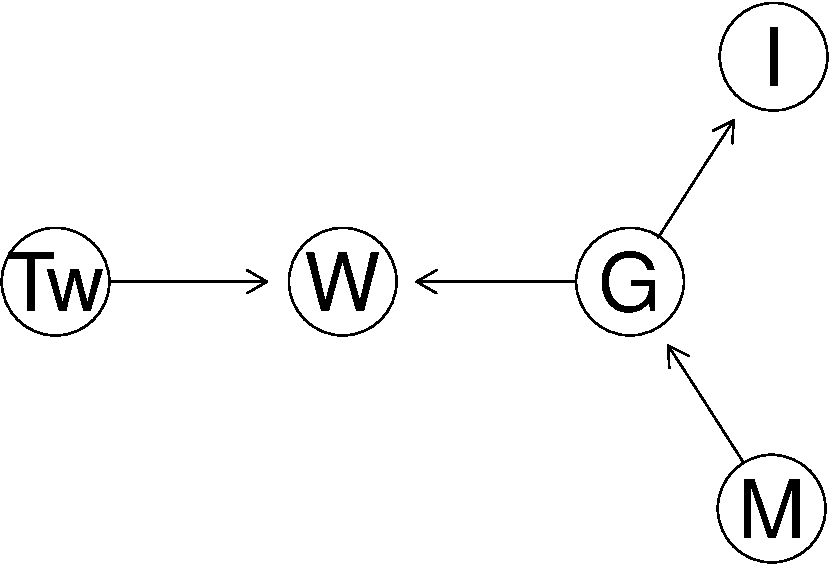
\includegraphics[width=1\linewidth]{coherencePaperRevised_files/figure-latex/unnamed-chunk-12-1} \end{center}
\end{subfigure}} \hfill
\hspace{-3cm}\begin{subfigure}[!ht]{0.7\textwidth}
\begin{table}[H]
\centering
\begin{tabular}{lr}
\toprule
B & Pr\\
\midrule
\cellcolor{gray!6}{1} & \cellcolor{gray!6}{0.5}\\
0 & 0.5\\
\bottomrule
\end{tabular}
\end{table}

\begin{table}[H]
\centering
\begin{tabular}{lrr}
\toprule
\multicolumn{1}{c}{P} & \multicolumn{2}{c}{B} \\
  & 1 & 0\\
\midrule
\cellcolor{gray!6}{1} & \cellcolor{gray!6}{0.02} & \cellcolor{gray!6}{0}\\
0 & 0.98 & 1\\
\bottomrule
\end{tabular}
\end{table}

\begin{table}[H]
\centering
\begin{tabular}{lllr}
\toprule
\multicolumn{1}{c}{} & \multicolumn{1}{c}{B} & \multicolumn{1}{c}{P} & \multicolumn{1}{c}{} \\
G &  &  & Pr\\
\midrule
\cellcolor{gray!6}{1} & \cellcolor{gray!6}{1} & \cellcolor{gray!6}{1} & \cellcolor{gray!6}{1.00}\\
0 & 1 & 1 & 0.00\\
\cellcolor{gray!6}{1} & \cellcolor{gray!6}{0} & \cellcolor{gray!6}{1} & \cellcolor{gray!6}{0.00}\\
0 & 0 & 1 & 1.00\\
\cellcolor{gray!6}{1} & \cellcolor{gray!6}{1} & \cellcolor{gray!6}{0} & \cellcolor{gray!6}{0.00}\\
0 & 1 & 0 & 1.00\\
\cellcolor{gray!6}{1} & \cellcolor{gray!6}{0} & \cellcolor{gray!6}{0} & \cellcolor{gray!6}{0.98}\\
0 & 0 & 0 & 0.02\\
\bottomrule
\end{tabular}
\end{table}
\end{subfigure}
\caption{Bayesian network for the \textsf{BGP} scenario.}
\label{fig:BGP}
\end{figure}

\begin{figure}
\hspace{2cm}\scalebox{0.6}{
\begin{subfigure}[!ht]{0.4\textwidth}

\begin{center}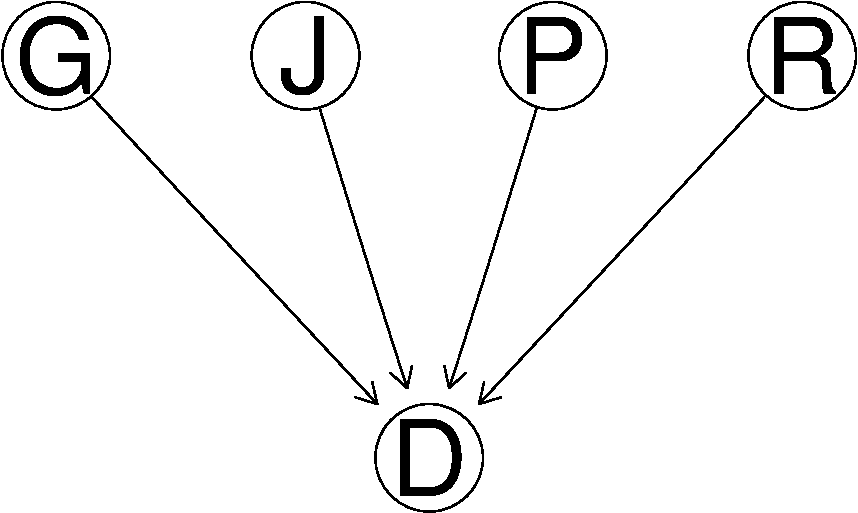
\includegraphics[width=0.7\linewidth]{coherencePaperRevised_files/figure-latex/unnamed-chunk-14-1} \end{center}
\end{subfigure} }
\hfill
\hspace{-3cm}\begin{subfigure}[!ht]{0.7\textwidth}
\begin{table}[H]
\centering
\begin{tabular}{lr}
\toprule
B & Pr\\
\midrule
\cellcolor{gray!6}{1} & \cellcolor{gray!6}{0.5}\\
0 & 0.5\\
\bottomrule
\end{tabular}
\end{table}

\begin{table}[H]
\centering
\begin{tabular}{lrr}
\toprule
\multicolumn{1}{c}{G} & \multicolumn{2}{c}{B} \\
  & 1 & 0\\
\midrule
\cellcolor{gray!6}{1} & \cellcolor{gray!6}{0.02} & \cellcolor{gray!6}{0.98}\\
0 & 0.98 & 0.02\\
\bottomrule
\end{tabular}
\end{table}
\end{subfigure}
\label{fig-BG}
\caption{Bayesian network for the \textsf{BG} scenario.}
\end{figure}

\begin{figure}
\scalebox{0.6}{
\hspace{4cm}\begin{subfigure}[!ht]{0.4\textwidth}

\begin{center}
\includegraphics{coherencePaperRevised_files/figure-latex/unnamed-chunk-16-1} \end{center}
\end{subfigure}} \hfill
\hspace{-3cm}\begin{subfigure}[!ht]{0.7\textwidth}
\begin{table}[H]
\centering
\begin{tabular}{lr}
\toprule
B & Pr\\
\midrule
\cellcolor{gray!6}{1} & \cellcolor{gray!6}{0.5}\\
0 & 0.5\\
\bottomrule
\end{tabular}
\end{table}

\begin{table}[H]
\centering
\begin{tabular}{lrr}
\toprule
\multicolumn{1}{c}{P} & \multicolumn{2}{c}{B} \\
  & 1 & 0\\
\midrule
\cellcolor{gray!6}{1} & \cellcolor{gray!6}{0.02} & \cellcolor{gray!6}{0}\\
0 & 0.98 & 1\\
\bottomrule
\end{tabular}
\end{table}
\end{subfigure}
\caption{Bayesian network for the \textsf{BP} scenario.}
\label{fig:BP}
\end{figure}\newpage 

Now, let's calculate the coherences and see if the desiderata are
satisfied (the abbreviations we already used are as before, and
\textsf{S} stands for \emph{Structured}, our coherence measure):

\begin{table}[H]
\centering
\resizebox{\linewidth}{!}{
\begin{tabular}{lrrrrrrrr}
\toprule
  & OG & OGen & Sh & ShGen & Fit & DM & R & S\\
\midrule
\cellcolor{gray!6}{Penguins: BGP 111} & \cellcolor{gray!6}{0.01} & \cellcolor{gray!6}{0.015} & \cellcolor{gray!6}{4.00} & \cellcolor{gray!6}{2.01} & \cellcolor{gray!6}{0.453} & \cellcolor{gray!6}{0.255} & \cellcolor{gray!6}{0.255} & \cellcolor{gray!6}{0.01}\\
Penguins: BG 11 & 0.01 & 0.010 & 0.04 & 0.04 & -0.960 & -0.480 & -0.480 & -0.96\\
\cellcolor{gray!6}{Penguins: BP 11} & \cellcolor{gray!6}{0.02} & \cellcolor{gray!6}{0.020} & \cellcolor{gray!6}{2.00} & \cellcolor{gray!6}{2.00} & \cellcolor{gray!6}{0.669} & \cellcolor{gray!6}{0.255} & \cellcolor{gray!6}{0.255} & \cellcolor{gray!6}{0.01}\\
\bottomrule
\end{tabular}}
\end{table}

\begin{table}[H]
\centering
\resizebox{\linewidth}{!}{
\begin{tabular}{lllllllll}
\toprule
  & OG & OGen & Sh & ShGen & Fit & DM & R & S\\
\midrule
\cellcolor{gray!6}{Penguins: BG$<$BGP} & \cellcolor{gray!6}{FALSE} & \cellcolor{gray!6}{TRUE} & \cellcolor{gray!6}{TRUE} & \cellcolor{gray!6}{TRUE} & \cellcolor{gray!6}{TRUE} & \cellcolor{gray!6}{TRUE} & \cellcolor{gray!6}{TRUE} & \cellcolor{gray!6}{TRUE}\\
Penguins: BP$\approx$ BGP & TRUE & TRUE & FALSE & TRUE & FALSE & TRUE & TRUE & TRUE\\
\bottomrule
\end{tabular}}
\end{table}

\subsection{Dunnit}\label{dunnit-1}

Here, we deal with two separate BNs. One, before the \textsf{Twin} node
is even considered (Fig. \ref{fig:twinless}), and one with the
\textsf{Twin} node (Fig. \ref{fig:twin}).

The CPTs for the no-twin version are in agreement with those in the ones
in the Twin case. Since the original example didn't specify exact
probabilities, we came up with some plausible values.

\begin{figure}

\scalebox{1.7}{
\begin{subfigure}[!ht]{0.3\textwidth}

\begin{center}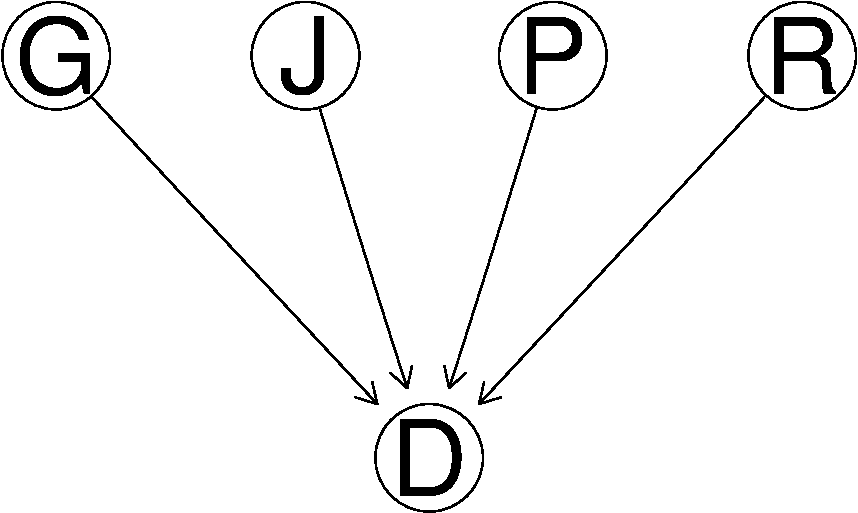
\includegraphics[width=0.7\linewidth]{coherencePaperRevised_files/figure-latex/unnamed-chunk-19-1} \end{center}
\end{subfigure}} 
\hspace{-0.8cm}\begin{subfigure}[!ht]{0.2\textwidth}
\begin{table}[H]
\centering
\begin{tabular}{lr}
\toprule
M & Pr\\
\midrule
\cellcolor{gray!6}{1} & \cellcolor{gray!6}{0.4}\\
0 & 0.6\\
\bottomrule
\end{tabular}
\end{table}

\begin{table}[H]
\centering
\begin{tabular}{lrr}
\toprule
\multicolumn{1}{c}{G} & \multicolumn{2}{c}{M} \\
  & 1 & 0\\
\midrule
\cellcolor{gray!6}{1} & \cellcolor{gray!6}{0.05} & \cellcolor{gray!6}{0.005}\\
0 & 0.95 & 0.995\\
\bottomrule
\end{tabular}
\end{table}
\end{subfigure}  
 \hspace{0.5cm}\begin{subfigure}[!ht]{0.2\textwidth}
\begin{table}[H]
\centering
\begin{tabular}{lrr}
\toprule
\multicolumn{1}{c}{I} & \multicolumn{2}{c}{G} \\
  & 1 & 0\\
\midrule
\cellcolor{gray!6}{1} & \cellcolor{gray!6}{0.8} & \cellcolor{gray!6}{0.005}\\
0 & 0.2 & 0.995\\
\bottomrule
\end{tabular}
\end{table}

\begin{table}[H]
\centering
\begin{tabular}{lrr}
\toprule
\multicolumn{1}{c}{W} & \multicolumn{2}{c}{G} \\
  & 1 & 0\\
\midrule
\cellcolor{gray!6}{1} & \cellcolor{gray!6}{0.012} & \cellcolor{gray!6}{0.207}\\
0 & 0.988 & 0.793\\
\bottomrule
\end{tabular}
\end{table}
\end{subfigure}
\caption{Twin-less BN for the \textsf{Dunnit} problem.}
\label{fig:twinless}
\end{figure}

\begin{figure}
\scalebox{1.7}{
\begin{subfigure}[!ht]{0.4\textwidth}

\begin{center}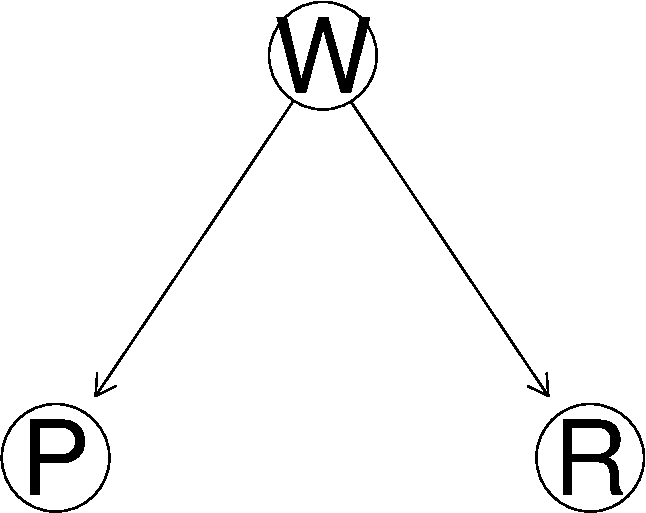
\includegraphics[width=0.7\linewidth]{coherencePaperRevised_files/figure-latex/unnamed-chunk-22-1} \end{center}
\end{subfigure}} 
\hspace{-1cm}\begin{subfigure}[!ht]{0.3\textwidth}
\begin{table}[H]
\centering
\begin{tabular}{lllr}
\toprule
\multicolumn{1}{c}{} & \multicolumn{1}{c}{G} & \multicolumn{1}{c}{Tw} & \multicolumn{1}{c}{} \\
W &  &  & Pr\\
\midrule
\cellcolor{gray!6}{1} & \cellcolor{gray!6}{1} & \cellcolor{gray!6}{1} & \cellcolor{gray!6}{0.200}\\
0 & 1 & 1 & 0.800\\
\cellcolor{gray!6}{1} & \cellcolor{gray!6}{0} & \cellcolor{gray!6}{1} & \cellcolor{gray!6}{0.400}\\
0 & 0 & 1 & 0.600\\
\cellcolor{gray!6}{1} & \cellcolor{gray!6}{1} & \cellcolor{gray!6}{0} & \cellcolor{gray!6}{0.005}\\
0 & 1 & 0 & 0.995\\
\cellcolor{gray!6}{1} & \cellcolor{gray!6}{0} & \cellcolor{gray!6}{0} & \cellcolor{gray!6}{0.200}\\
0 & 0 & 0 & 0.800\\
\bottomrule
\end{tabular}
\end{table}
\end{subfigure}
\caption{BN for the \textsf{Dunnit} problem. The key difference for the twin version lies in the construction of the CPT for \textsf{W}. The table gives conditional probabilities for \textsf{W} given various joint states of \textsf{Tw} and \textsf{G}.}
\label{fig:twin}
\end{figure}

\newpage

Coherence calculations result in the following:

\begin{table}[H]
\centering
\resizebox{\linewidth}{!}{
\begin{tabular}{lrrrrrrrr}
\toprule
  & OG & OGen & Sh & ShGen & Fit & DM & R & S\\
\midrule
\cellcolor{gray!6}{Dunnit: MGWI 1111} & \cellcolor{gray!6}{0} & \cellcolor{gray!6}{0.087} & \cellcolor{gray!6}{4.294} & \cellcolor{gray!6}{11.012} & \cellcolor{gray!6}{0.169} & \cellcolor{gray!6}{0.167} & \cellcolor{gray!6}{0.167} & \cellcolor{gray!6}{-0.932}\\
Dunnit: MTGWI 11111 & 0 & 0.042 & 73.836 & 13.669 & 0.385 & 0.150 & 0.150 & -0.100\\
\bottomrule
\end{tabular}}
\end{table}

\begin{table}[H]
\centering
\resizebox{\linewidth}{!}{
\begin{tabular}{lllllllll}
\toprule
  & OG & OGen & Sh & ShGen & Fit & DM & R & S\\
\midrule
\cellcolor{gray!6}{Dunnit: Dunnit$<$Twin} & \cellcolor{gray!6}{FALSE} & \cellcolor{gray!6}{FALSE} & \cellcolor{gray!6}{TRUE} & \cellcolor{gray!6}{TRUE} & \cellcolor{gray!6}{TRUE} & \cellcolor{gray!6}{FALSE} & \cellcolor{gray!6}{FALSE} & \cellcolor{gray!6}{TRUE}\\
\bottomrule
\end{tabular}}
\end{table}

\subsection{Japanese swords}\label{japanese-swords-1}

There is a common DAG for the three scenarios, but the CPTs differ (Fig.
\ref{fig:japanese}).

\begin{figure}
\scalebox{0.5}{
\hspace{2.5cm}\begin{subfigure}[!ht]{0.4\textwidth}

\begin{center}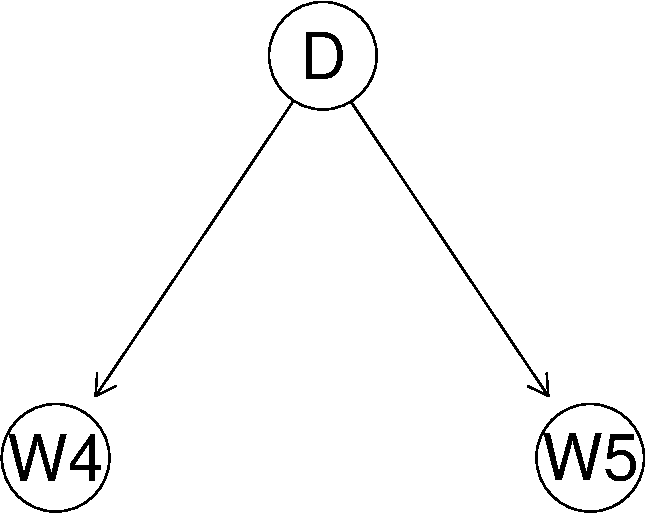
\includegraphics[width=0.7\linewidth]{coherencePaperRevised_files/figure-latex/unnamed-chunk-25-1} \end{center}
\end{subfigure}} \hfill
\begin{subfigure}[!ht]{0.6\textwidth}
\begin{table}[H]
\centering
\begin{tabular}{lr}
\toprule
J & Pr\\
\midrule
\cellcolor{gray!6}{1} & \cellcolor{gray!6}{0}\\
0 & 1\\
\bottomrule
\end{tabular}
\end{table}

\begin{table}[H]
\centering
\begin{tabular}{lrr}
\toprule
\multicolumn{1}{c}{O} & \multicolumn{2}{c}{J} \\
  & 1 & 0\\
\midrule
\cellcolor{gray!6}{1} & \cellcolor{gray!6}{0.008} & \cellcolor{gray!6}{0}\\
0 & 0.992 & 1\\
\bottomrule
\end{tabular}
\end{table}
\caption{Scenario 1.}
\end{subfigure} 
\begin{subfigure}[!ht]{0.4\textwidth}
\begin{table}[H]
\centering
\begin{tabular}{lr}
\toprule
J & Pr\\
\midrule
\cellcolor{gray!6}{1} & \cellcolor{gray!6}{0.1}\\
0 & 0.9\\
\bottomrule
\end{tabular}
\end{table}

\begin{table}[H]
\centering
\begin{tabular}{lrr}
\toprule
\multicolumn{1}{c}{O} & \multicolumn{2}{c}{J} \\
  & 1 & 0\\
\midrule
\cellcolor{gray!6}{1} & \cellcolor{gray!6}{0.9} & \cellcolor{gray!6}{0.011}\\
0 & 0.1 & 0.989\\
\bottomrule
\end{tabular}
\end{table}
\caption{Scenario 2.}
\end{subfigure}  \hfill
\begin{subfigure}[!ht]{0.6\textwidth}
\begin{table}[H]
\centering
\begin{tabular}{lr}
\toprule
J & Pr\\
\midrule
\cellcolor{gray!6}{1} & \cellcolor{gray!6}{0.833}\\
0 & 0.167\\
\bottomrule
\end{tabular}
\end{table}

\begin{table}[H]
\centering
\begin{tabular}{lrr}
\toprule
\multicolumn{1}{c}{O} & \multicolumn{2}{c}{J} \\
  & 1 & 0\\
\midrule
\cellcolor{gray!6}{1} & \cellcolor{gray!6}{0.9} & \cellcolor{gray!6}{0.5}\\
0 & 0.1 & 0.5\\
\bottomrule
\end{tabular}
\end{table}
\caption{Scenario 3.}
\end{subfigure} 
\caption{A common DAG and three sets of CPTs for the \textsf{Japanese Swords} problem.}
\label{fig:japanese}
\end{figure}

\newpage 

Coherence calculations yield:

\begin{table}[H]
\centering
\resizebox{\linewidth}{!}{
\begin{tabular}{lrrrrrrrr}
\toprule
  & OG & OGen & Sh & ShGen & Fit & DM & R & S\\
\midrule
\cellcolor{gray!6}{Japanese Swords 1: JO 11} & \cellcolor{gray!6}{0.004} & \cellcolor{gray!6}{0.004} & \cellcolor{gray!6}{80.251} & \cellcolor{gray!6}{80.251} & \cellcolor{gray!6}{0.976} & \cellcolor{gray!6}{0.008} & \cellcolor{gray!6}{0.008} & \cellcolor{gray!6}{0.008}\\
Japanese Swords 2: JO 11 & 0.818 & 0.818 & 9.000 & 9.000 & 0.976 & 0.800 & 0.800 & 0.889\\
\cellcolor{gray!6}{Japanese Swords 3: JO 11} & \cellcolor{gray!6}{0.818} & \cellcolor{gray!6}{0.818} & \cellcolor{gray!6}{1.080} & \cellcolor{gray!6}{1.080} & \cellcolor{gray!6}{0.286} & \cellcolor{gray!6}{0.067} & \cellcolor{gray!6}{0.067} & \cellcolor{gray!6}{0.400}\\
\bottomrule
\end{tabular}}
\end{table}

\begin{table}[H]
\centering
\resizebox{\linewidth}{!}{
\begin{tabular}{lllllllll}
\toprule
  & OG & OGen & Sh & ShGen & Fit & DM & R & S\\
\midrule
\cellcolor{gray!6}{Swords: JO2$>$JO1} & \cellcolor{gray!6}{TRUE} & \cellcolor{gray!6}{TRUE} & \cellcolor{gray!6}{FALSE} & \cellcolor{gray!6}{FALSE} & \cellcolor{gray!6}{TRUE} & \cellcolor{gray!6}{TRUE} & \cellcolor{gray!6}{TRUE} & \cellcolor{gray!6}{TRUE}\\
Swords: JO2$>$JO3 & FALSE & FALSE & TRUE & TRUE & TRUE & TRUE & TRUE & TRUE\\
\bottomrule
\end{tabular}}
\end{table}

\subsection{Robbers}\label{robbers-1}

The robbers counterexample involves a phenomenon we've already seen: it
is not clear whether the information about the prior probabilities is
supposed to be part of the narration or not. If we want to include this
information in our coherence assessment, we can do this employing a
single BN.

\begin{figure}
\begin{subfigure}[!ht]{0.4\textwidth}

\begin{center}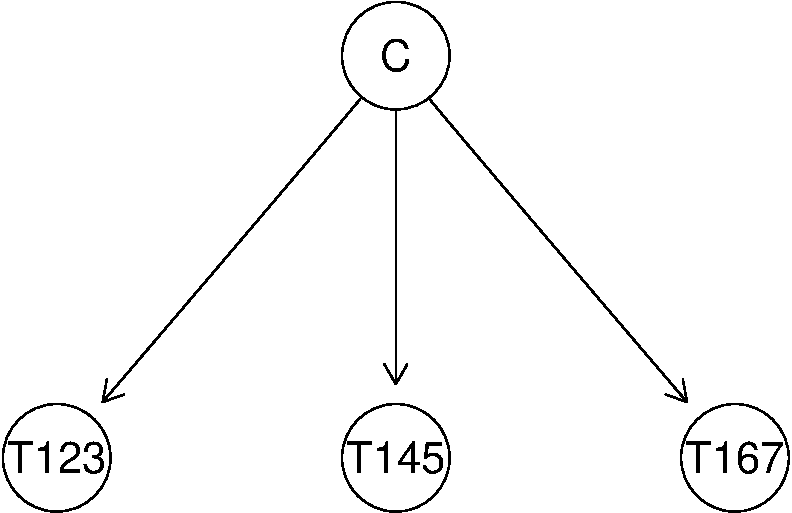
\includegraphics{coherencePaperRevised_files/figure-latex/unnamed-chunk-30-1} \end{center}
\end{subfigure} \hfill
\begin{subfigure}[!ht]{0.6\textwidth}
\begin{table}[H]
\centering\begingroup\fontsize{9}{11}\selectfont

\begin{tabular}{lr}
\toprule
  & Pr\\
\midrule
\cellcolor{gray!6}{OnlyP} & \cellcolor{gray!6}{0.2}\\
OnlyR & 0.2\\
\cellcolor{gray!6}{Both} & \cellcolor{gray!6}{0.6}\\
\bottomrule
\end{tabular}
\endgroup{}
\end{table}

\begin{table}[H]
\centering\begingroup\fontsize{9}{11}\selectfont

\begin{tabular}{lrrr}
\toprule
\multicolumn{1}{c}{MisP} & \multicolumn{3}{c}{WhoMurdered} \\
  & OnlyP & OnlyR & Both\\
\midrule
\cellcolor{gray!6}{1} & \cellcolor{gray!6}{1} & \cellcolor{gray!6}{0} & \cellcolor{gray!6}{1}\\
0 & 0 & 1 & 0\\
\bottomrule
\end{tabular}
\endgroup{}
\end{table}

\begin{table}[H]
\centering\begingroup\fontsize{9}{11}\selectfont

\begin{tabular}{lrrr}
\toprule
\multicolumn{1}{c}{MisR} & \multicolumn{3}{c}{WhoMurdered} \\
  & OnlyP & OnlyR & Both\\
\midrule
\cellcolor{gray!6}{1} & \cellcolor{gray!6}{0} & \cellcolor{gray!6}{1} & \cellcolor{gray!6}{1}\\
0 & 1 & 0 & 0\\
\bottomrule
\end{tabular}
\endgroup{}
\end{table}
\end{subfigure}
\caption{BN for the \textsf{Robbers} problem.}
\label{fig:Robbers}
\end{figure}

\newpage

Coherence calculations yield the following results:

\begin{table}[H]
\centering
\resizebox{\linewidth}{!}{
\begin{tabular}{lrrrrrrrr}
\toprule
  & OG & OGen & Sh & ShGen & Fit & DM & R & S\\
\midrule
Robbers: MIsPMIsR 11 & 0.60 & 0.60 & 0.937 & 0.937 & -0.143 & -0.050 & -0.050 & 0.6\\
Robbers: MIsPMIsR 10 & 0.25 & 0.25 & 1.250 & 1.250 & 0.571 & 0.125 & 0.125 & -0.6\\
Robbers: MIsPMIsR 01 & 0.25 & 0.25 & 1.250 & 1.250 & 0.571 & 0.125 & 0.125 & -0.6\\
\bottomrule
\end{tabular}}
\end{table}

\begin{table}[H]
\centering
\resizebox{\linewidth}{!}{
\begin{tabular}{lllllllll}
\toprule
  & OG & OGen & Sh & ShGen & Fit & DM & R & S\\
\midrule
Robbers: PR$>$P$\neg$R & TRUE & TRUE & FALSE & FALSE & FALSE & FALSE & FALSE & TRUE\\
Robbers: PR$>$neutral & NA & NA & FALSE & FALSE & FALSE & FALSE & FALSE & TRUE\\
\bottomrule
\end{tabular}}
\end{table}

\subsection{The Beatles}\label{the-beatles-1}

\begin{figure}
\scalebox{1.6}{
\begin{subfigure}[!ht]{0.4\textwidth}

\begin{center}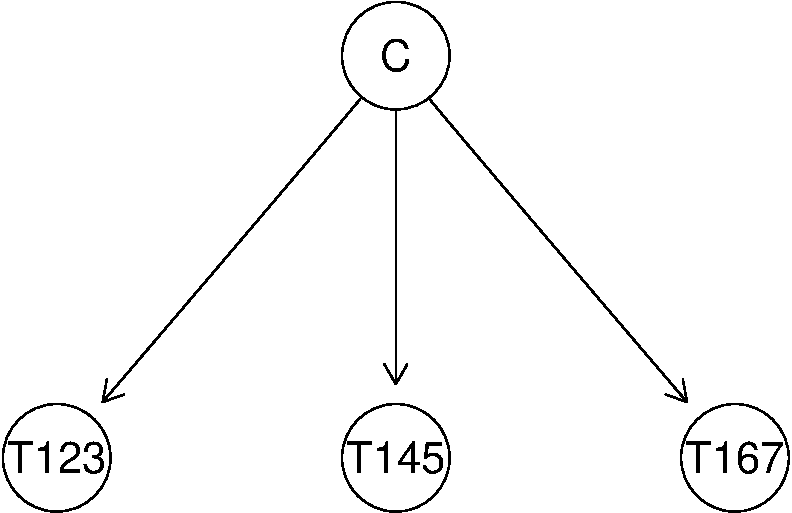
\includegraphics[width=0.7\linewidth]{coherencePaperRevised_files/figure-latex/unnamed-chunk-33-1} \end{center}
\end{subfigure}} \hfill
\begin{subfigure}[!ht]{0.4\textwidth}
\begin{table}[H]
\centering
\begin{tabular}{lr}
\toprule
G & Pr\\
\midrule
\cellcolor{gray!6}{1} & \cellcolor{gray!6}{0.5}\\
0 & 0.5\\
\bottomrule
\end{tabular}
\end{table}
\end{subfigure}
\caption{Bayesian network for the \textsf{Beatles} scenario.}
\end{figure}

We assume the prior probability of each individual band member being
dead to 0.5 (as in the above table), and the CPT for \textsf{D} is
many-dimensional and so difficult to present concisely, but the method
is straigtforward: probability 1 is given to \textsf{D} in all
combinations of the parents in which exactly one is true, and otherwise
\textsf{D} gets conditional probability 0. Coherence calculations give
the following results:

\begin{table}[H]
\centering
\resizebox{\linewidth}{!}{
\begin{tabular}{lrrrrrrrr}
\toprule
  & OG & OGen & Sh & ShGen & Fit & DM & R & S\\
\midrule
\cellcolor{gray!6}{Beatles: JPGRD 11111} & \cellcolor{gray!6}{0} & \cellcolor{gray!6}{0.202} & \cellcolor{gray!6}{0} & \cellcolor{gray!6}{1.423} & \cellcolor{gray!6}{-0.036} & \cellcolor{gray!6}{0.025} & \cellcolor{gray!6}{0.025} & \cellcolor{gray!6}{-1}\\
\bottomrule
\end{tabular}}
\end{table}

\begin{table}[H]
\centering
\resizebox{\linewidth}{!}{
\begin{tabular}{lllllllll}
\toprule
  & OG & OGen & Sh & ShGen & Fit & DM & R & S\\
\midrule
\cellcolor{gray!6}{Beatles: below neutral} & \cellcolor{gray!6}{NA} & \cellcolor{gray!6}{NA} & \cellcolor{gray!6}{TRUE} & \cellcolor{gray!6}{FALSE} & \cellcolor{gray!6}{TRUE} & \cellcolor{gray!6}{FALSE} & \cellcolor{gray!6}{TRUE} & \cellcolor{gray!6}{TRUE}\\
Beatles: minimal & TRUE & FALSE & TRUE & FALSE & FALSE & FALSE & FALSE & TRUE\\
\bottomrule
\end{tabular}}
\end{table}

\subsection{Alicja and books}\label{alicja-and-books-1}

The BN is fairly straightforward (Fig. \ref{fig:books}) and the results
are as follows:

\begin{figure}

\hspace{20mm}
\scalebox{0.5}{\begin{subfigure}[!ht]{0.4\textwidth}

\begin{center}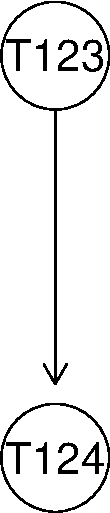
\includegraphics{coherencePaperRevised_files/figure-latex/unnamed-chunk-36-1} \end{center}
\end{subfigure}} \hfill
\begin{subfigure}[!ht]{0.6\textwidth}
\begin{table}[H]
\centering
\begin{tabular}{lr}
\toprule
A & Pr\\
\midrule
\cellcolor{gray!6}{1} & \cellcolor{gray!6}{0.01}\\
0 & 0.99\\
\bottomrule
\end{tabular}
\end{table}

\begin{table}[H]
\centering
\begin{tabular}{lrr}
\toprule
\multicolumn{1}{c}{R} & \multicolumn{2}{c}{A} \\
  & 1 & 0\\
\midrule
\cellcolor{gray!6}{1} & \cellcolor{gray!6}{0.15} & \cellcolor{gray!6}{0.1}\\
0 & 0.85 & 0.9\\
\bottomrule
\end{tabular}
\end{table}
\end{subfigure}
\caption{Bayesian network for the \textsf{Books} problem.}
\label{fig:books}
\end{figure}

\begin{table}[H]
\centering
\resizebox{\linewidth}{!}{
\begin{tabular}{lrrrrrrrr}
\toprule
  & OG & OGen & Sh & ShGen & Fit & DM & R & S\\
\midrule
\cellcolor{gray!6}{Books: AR 11} & \cellcolor{gray!6}{0.014} & \cellcolor{gray!6}{0.014} & \cellcolor{gray!6}{1.493} & \cellcolor{gray!6}{1.493} & \cellcolor{gray!6}{0.212} & \cellcolor{gray!6}{0.027} & \cellcolor{gray!6}{0.027} & \cellcolor{gray!6}{0.055}\\
Books: AR 10 & 0.009 & 0.009 & 0.945 & 0.945 & -0.127 & -0.025 & -0.025 & -0.055\\
\cellcolor{gray!6}{Books: AR 01} & \cellcolor{gray!6}{0.100} & \cellcolor{gray!6}{0.100} & \cellcolor{gray!6}{0.995} & \cellcolor{gray!6}{0.995} & \cellcolor{gray!6}{-0.101} & \cellcolor{gray!6}{-0.003} & \cellcolor{gray!6}{-0.003} & \cellcolor{gray!6}{-0.005}\\
Books: AR 00 & 0.892 & 0.892 & 1.001 & 1.001 & 0.016 & 0.001 & 0.001 & 0.005\\
\bottomrule
\end{tabular}}
\end{table}

\begin{table}[H]
\centering
\resizebox{\linewidth}{!}{
\begin{tabular}{lllllllll}
\toprule
  & OG & OGen & Sh & ShGen & Fit & DM & R & S\\
\midrule
\cellcolor{gray!6}{Books: AR$>$A$\neg$R} & \cellcolor{gray!6}{TRUE} & \cellcolor{gray!6}{TRUE} & \cellcolor{gray!6}{TRUE} & \cellcolor{gray!6}{TRUE} & \cellcolor{gray!6}{TRUE} & \cellcolor{gray!6}{TRUE} & \cellcolor{gray!6}{TRUE} & \cellcolor{gray!6}{TRUE}\\
Books: AR$>\neg$AR & FALSE & FALSE & TRUE & TRUE & TRUE & TRUE & TRUE & TRUE\\
\cellcolor{gray!6}{Books: $\neg$A$\neg$R$>$A$\neg$R} & \cellcolor{gray!6}{TRUE} & \cellcolor{gray!6}{TRUE} & \cellcolor{gray!6}{TRUE} & \cellcolor{gray!6}{TRUE} & \cellcolor{gray!6}{TRUE} & \cellcolor{gray!6}{TRUE} & \cellcolor{gray!6}{TRUE} & \cellcolor{gray!6}{TRUE}\\
Books: $\neg$A$\neg$R$>\neg$AR & TRUE & TRUE & TRUE & TRUE & TRUE & TRUE & TRUE & TRUE\\
\bottomrule
\end{tabular}}
\end{table}

\subsection{The witnesses}\label{the-witnesses-1}

Two requirements are associated with this example: both
\(\{\)\textsf{W1, W2}\(\}\) and \(\{\)\textsf{W4, W5}\(\}\) should be
more coherent than \(\{\)\textsf{W3, W4}\(\}\). The basic idea behind
the CPTs we used is that for any particular witness we take the
probability of them including the perpetrator in their list to be 0.8,
and the probability of including an innocent to be .05. Of course, the
example can be run with different conditional probability tables. Let's
first take a look at the BN for the first scenario (Fig.
\ref{fig:w1w2}).

\begin{figure}
\scalebox{1.2}{
\hspace{1cm}\begin{subfigure}[!ht]{0.4\textwidth}

\begin{center}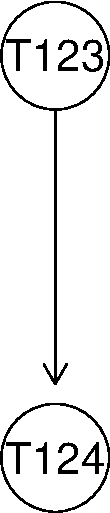
\includegraphics[width=1\linewidth]{coherencePaperRevised_files/figure-latex/unnamed-chunk-39-1} \end{center}
\end{subfigure}} \hfill
\begin{subfigure}[!ht]{0.3\textwidth}
\begin{table}[H]
\centering
\begin{tabular}{lr}
\toprule
D & Pr\\
\midrule
\cellcolor{gray!6}{Steve} & \cellcolor{gray!6}{0.167}\\
Martin & 0.167\\
\cellcolor{gray!6}{David} & \cellcolor{gray!6}{0.167}\\
John & 0.167\\
\cellcolor{gray!6}{James} & \cellcolor{gray!6}{0.167}\\
Peter & 0.167\\
\bottomrule
\end{tabular}
\end{table}
\end{subfigure}
\centering
\begin{subfigure}[!ht]{0.3\textwidth}
\begin{table}[H]
\centering\begin{table}[H]
\centering
\begin{tabular}{lrrrrrr}
\toprule
\multicolumn{1}{c}{W1} & \multicolumn{2}{c}{D} \\
  & Steve & Martin & David & John & James & Peter\\
\midrule
\cellcolor{gray!6}{\cellcolor{gray!6}{1}} & \cellcolor{gray!6}{\cellcolor{gray!6}{0.8}} & \cellcolor{gray!6}{\cellcolor{gray!6}{0.05}} & \cellcolor{gray!6}{\cellcolor{gray!6}{0.05}} & \cellcolor{gray!6}{\cellcolor{gray!6}{0.05}} & \cellcolor{gray!6}{\cellcolor{gray!6}{0.05}} & \cellcolor{gray!6}{\cellcolor{gray!6}{0.05}}\\
0 & 0.2 & 0.95 & 0.95 & 0.95 & 0.95 & 0.95\\
\bottomrule
\end{tabular}
\end{table}
\end{table}
\end{subfigure}
\caption{BN for the \textsf{W1W2} narration in the \textsf{Witness} problem. CPT for \textsf{W2} is identical to the one for \textsf{W1}.}
\label{fig:w1w2}
\end{figure}

The CPT for \textsf{D} is uniform. The table for \textsf{W1} provides
the conditional probability of \textsf{W1} listing (\textsf{W1}=1) or
not listing (\textsf{W1}=0) a particular person given that the actual
value of \textsf{D} is Steve/Martin/\dots. The underlying rule is: if
someone is guilty, a witness will mention them with probability \(.8\),
and if they aren't, they will be listed with probability \(.05\). In the
remaining two BNs for the problem the CPT for \textsf{D} remains the
same, and the CPTs for the witness nodes are analogous to the one for
\textsf{W1}. The remaining BNs have the following obvious DAGs (Fig.
\ref{fig:witness}).

\begin{figure}\centering
\scalebox{1.2}{
\begin{subfigure}[!ht]{0.4\textwidth}

\begin{center}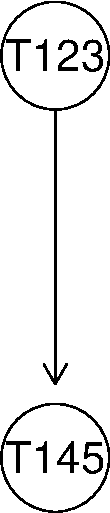
\includegraphics[width=1\linewidth]{coherencePaperRevised_files/figure-latex/unnamed-chunk-42-1} \end{center}
\end{subfigure}}

\scalebox{1.2}{\begin{subfigure}[!ht]{0.4\textwidth}

\begin{center}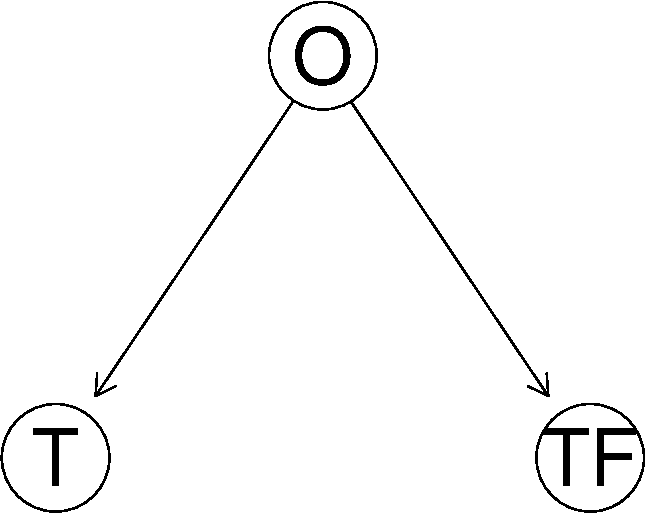
\includegraphics[width=1\linewidth]{coherencePaperRevised_files/figure-latex/unnamed-chunk-43-1} \end{center}
\end{subfigure}}
\caption{Two remaining DAGs for the \textsf{Witness} problem.}
\label{fig:witness}
\end{figure}

\newpage

We think that what this example illustrates is that we should really
carefully think about whose cognitive perspective is taken when we
represent a narration using a BN, focusing on whether the BN involves
nodes which are not part of the narration whose coherence is to be
evaluated. In particular, the probabilistic information about the
uniform distribution of guilt probability is not part of any of the
three involved narrations, but rather a part of a third-person set-up
prior to obtaining any evidence.

To evaluate the coherence of a narration, at least for unmentioned
assumptions that one doesn't have strong independent reasons to keep,
one should think counterfactually, granting the consequences of the
narration and asking what would happen if it indeed was true. In our
case, a judge who evaluates the coherence of witness testimonies once
she has heard them, no longer thinks that the distribution of \textsf{D}
is uniform. And this agrees with the counterfactual strategy we just
described: it is a consequence of the probabilistic set-up and the
content of \textsf{W1} and \textsf{W2} that if \textsf{W1} and
\textsf{W2} were true, the distribution for \textsf{D} no longer would
be uniform, and so it is unfair to judge the coherence of this scenario
without giving up this assumption and updating one's assumptions about
\textsf{D}.

In such a case, we think, we should update \textsf{D} to what it would
be had \textsf{W1} and \textsf{W2} be instantiated with 1s:

\begin{table}[H]
\centering
\begin{tabular}{lrrrrrr}
\toprule
  & Steve & Martin & David & John & James & Peter\\
\midrule
\cellcolor{gray!6}{Pr} & \cellcolor{gray!6}{0.981} & \cellcolor{gray!6}{0.004} & \cellcolor{gray!6}{0.004} & \cellcolor{gray!6}{0.004} & \cellcolor{gray!6}{0.004} & \cellcolor{gray!6}{0.004}\\
\bottomrule
\end{tabular}
\end{table}

\noindent and use these updated probabilities to build the weights used
in our coherence calculations for this narration (and proceed
accordingly, instead updating on another set of narration nodes in the
coherence evaluation of other
narrations).\footnote{Note  however that  you should not simply instantiate the BN with \textsf{W1} and \textsf{W2}, propagate and run the coherence calculations on the updated BN. Then both these nodes would get 1s in their respective CPTs and coherence calculations would make   all  confirmation measures involved in such calculations  based on posterior probability equal 1. If narration members have probability one, no other information will be able to confirm it.}
Once this strategy is taken, the problem turns out to be not that
challenging for any of the coherence measures under discussion.

\begin{table}[H]
\centering
\resizebox{\linewidth}{!}{
\begin{tabular}{lrrrrrrrr}
\toprule
  & OG & OGen & Sh & ShGen & Fit & DM & R & S\\
\midrule
\cellcolor{gray!6}{Witness: W1W2 11} & \cellcolor{gray!6}{0.451} & \cellcolor{gray!6}{0.451} & \cellcolor{gray!6}{3.551} & \cellcolor{gray!6}{3.551} & \cellcolor{gray!6}{0.771} & \cellcolor{gray!6}{0.446} & \cellcolor{gray!6}{0.446} & \cellcolor{gray!6}{0.729}\\
Witness: W3W4 11 & 0.187 & 0.187 & 0.740 & 0.740 & -0.234 & -0.110 & -0.110 & 0.494\\
\cellcolor{gray!6}{Witness: W4W5 11} & \cellcolor{gray!6}{0.365} & \cellcolor{gray!6}{0.365} & \cellcolor{gray!6}{1.260} & \cellcolor{gray!6}{1.260} & \cellcolor{gray!6}{0.218} & \cellcolor{gray!6}{0.110} & \cellcolor{gray!6}{0.110} & \cellcolor{gray!6}{0.602}\\
\bottomrule
\end{tabular}}
\end{table}

\begin{table}[H]
\centering
\resizebox{\linewidth}{!}{
\begin{tabular}{lllllllll}
\toprule
  & OG & OGen & Sh & ShGen & Fit & DM & R & S\\
\midrule
\cellcolor{gray!6}{Witness: W$_1$W$_2>$W$_3$W$_4$} & \cellcolor{gray!6}{TRUE} & \cellcolor{gray!6}{TRUE} & \cellcolor{gray!6}{TRUE} & \cellcolor{gray!6}{TRUE} & \cellcolor{gray!6}{TRUE} & \cellcolor{gray!6}{TRUE} & \cellcolor{gray!6}{TRUE} & \cellcolor{gray!6}{TRUE}\\
Witness: W$_4$W$_5>$W$_3$W$_4$ & TRUE & TRUE & TRUE & TRUE & TRUE & TRUE & TRUE & TRUE\\
\bottomrule
\end{tabular}}
\end{table}

\subsection{Depth}\label{depth-1}

We start with representing the two scenarios with two fairly natural BNs
(\textsf{C} stands for who Committed the crime, \textsf{TXYZ} stands for
Testimony that \(X\vee Y \vee Z\)), see Fig. \ref{fig:dod1} and
\ref{fig:dod2}.

\begin{figure}
\scalebox{1.7}{
\begin{subfigure}[!ht]{0.4\textwidth}

\begin{center}\includegraphics[width=0.7\linewidth]{coherencePaperRevised_files/figure-latex/unnamed-chunk-46-1} \end{center}
\end{subfigure}} 
\hspace{-1cm}\scalebox{0.6}{\begin{subfigure}[!ht]{0.3\textwidth}
\begin{table}[H]
\centering
\begin{tabular}{lr}
\toprule
C & Pr\\
\midrule
\cellcolor{gray!6}{1} & \cellcolor{gray!6}{0.125}\\
2 & 0.125\\
\cellcolor{gray!6}{3} & \cellcolor{gray!6}{0.125}\\
4 & 0.125\\
\cellcolor{gray!6}{5} & \cellcolor{gray!6}{0.125}\\
6 & 0.125\\
\cellcolor{gray!6}{7} & \cellcolor{gray!6}{0.125}\\
8 & 0.125\\
\bottomrule
\end{tabular}
\end{table}

\begin{table}[H]
\centering
\begin{tabular}{lrrrrrrrr}
\toprule
\multicolumn{1}{c}{T123} & \multicolumn{2}{c}{C} \\
  & 1 & 2 & 3 & 4 & 5 & 6 & 7 & 8\\
\midrule
\cellcolor{gray!6}{1} & \cellcolor{gray!6}{1} & \cellcolor{gray!6}{1} & \cellcolor{gray!6}{1} & \cellcolor{gray!6}{0} & \cellcolor{gray!6}{0} & \cellcolor{gray!6}{0} & \cellcolor{gray!6}{0} & \cellcolor{gray!6}{0}\\
0 & 0 & 0 & 0 & 1 & 1 & 1 & 1 & 1\\
\bottomrule
\end{tabular}
\end{table}

\begin{table}[H]
\centering
\begin{tabular}{lrrrrrrrr}
\toprule
\multicolumn{1}{c}{T124} & \multicolumn{2}{c}{C} \\
  & 1 & 2 & 3 & 4 & 5 & 6 & 7 & 8\\
\midrule
\cellcolor{gray!6}{1} & \cellcolor{gray!6}{1} & \cellcolor{gray!6}{1} & \cellcolor{gray!6}{0} & \cellcolor{gray!6}{1} & \cellcolor{gray!6}{0} & \cellcolor{gray!6}{0} & \cellcolor{gray!6}{0} & \cellcolor{gray!6}{0}\\
0 & 0 & 0 & 1 & 0 & 1 & 1 & 1 & 1\\
\bottomrule
\end{tabular}
\end{table}

\begin{table}[H]
\centering
\begin{tabular}{lrrrrrrrr}
\toprule
\multicolumn{1}{c}{T134} & \multicolumn{2}{c}{C} \\
  & 1 & 2 & 3 & 4 & 5 & 6 & 7 & 8\\
\midrule
\cellcolor{gray!6}{1} & \cellcolor{gray!6}{1} & \cellcolor{gray!6}{0} & \cellcolor{gray!6}{1} & \cellcolor{gray!6}{1} & \cellcolor{gray!6}{0} & \cellcolor{gray!6}{0} & \cellcolor{gray!6}{0} & \cellcolor{gray!6}{0}\\
0 & 0 & 1 & 0 & 0 & 1 & 1 & 1 & 1\\
\bottomrule
\end{tabular}
\end{table}
\end{subfigure}}
\caption{BN for \textsf{X1} in the \textsf{Depth} problem.}
\label{fig:dod1}
\end{figure}

\begin{figure}
\scalebox{1.7}{
\begin{subfigure}[!ht]{0.4\textwidth}

\begin{center}\includegraphics[width=0.7\linewidth]{coherencePaperRevised_files/figure-latex/unnamed-chunk-48-1} \end{center}
\end{subfigure}} 
\hspace{-1cm}\scalebox{0.6}{\begin{subfigure}[!ht]{0.3\textwidth}
\begin{table}[H]
\centering
\begin{tabular}{lr}
\toprule
C & Pr\\
\midrule
\cellcolor{gray!6}{1} & \cellcolor{gray!6}{0.125}\\
2 & 0.125\\
\cellcolor{gray!6}{3} & \cellcolor{gray!6}{0.125}\\
4 & 0.125\\
\cellcolor{gray!6}{5} & \cellcolor{gray!6}{0.125}\\
6 & 0.125\\
\cellcolor{gray!6}{7} & \cellcolor{gray!6}{0.125}\\
8 & 0.125\\
\bottomrule
\end{tabular}
\end{table}

\begin{table}[H]
\centering
\begin{tabular}{lrrrrrrrr}
\toprule
\multicolumn{1}{c}{T123} & \multicolumn{2}{c}{C} \\
  & 1 & 2 & 3 & 4 & 5 & 6 & 7 & 8\\
\midrule
\cellcolor{gray!6}{1} & \cellcolor{gray!6}{1} & \cellcolor{gray!6}{1} & \cellcolor{gray!6}{1} & \cellcolor{gray!6}{0} & \cellcolor{gray!6}{0} & \cellcolor{gray!6}{0} & \cellcolor{gray!6}{0} & \cellcolor{gray!6}{0}\\
0 & 0 & 0 & 0 & 1 & 1 & 1 & 1 & 1\\
\bottomrule
\end{tabular}
\end{table}

\begin{table}[H]
\centering
\begin{tabular}{lrrrrrrrr}
\toprule
\multicolumn{1}{c}{T145} & \multicolumn{2}{c}{C} \\
  & 1 & 2 & 3 & 4 & 5 & 6 & 7 & 8\\
\midrule
\cellcolor{gray!6}{1} & \cellcolor{gray!6}{1} & \cellcolor{gray!6}{0} & \cellcolor{gray!6}{0} & \cellcolor{gray!6}{1} & \cellcolor{gray!6}{1} & \cellcolor{gray!6}{0} & \cellcolor{gray!6}{0} & \cellcolor{gray!6}{0}\\
0 & 0 & 1 & 1 & 0 & 0 & 1 & 1 & 1\\
\bottomrule
\end{tabular}
\end{table}

\begin{table}[H]
\centering
\begin{tabular}{lrrrrrrrr}
\toprule
\multicolumn{1}{c}{T167} & \multicolumn{2}{c}{C} \\
  & 1 & 2 & 3 & 4 & 5 & 6 & 7 & 8\\
\midrule
\cellcolor{gray!6}{1} & \cellcolor{gray!6}{1} & \cellcolor{gray!6}{0} & \cellcolor{gray!6}{0} & \cellcolor{gray!6}{0} & \cellcolor{gray!6}{0} & \cellcolor{gray!6}{1} & \cellcolor{gray!6}{1} & \cellcolor{gray!6}{0}\\
0 & 0 & 1 & 1 & 1 & 1 & 0 & 0 & 1\\
\bottomrule
\end{tabular}
\end{table}
\end{subfigure}}
\caption{BN for \textsf{X2} in the \textsf{Depth} problem.}
\label{fig:dod2}
\end{figure}

\newpage

One effect of dropping the ``the witness testified that'' and using the
testimony contents themselves is that the CPTs for the narration nodes
are deterministically connected with the root node. In result, the
coherence calculations give in the following:

\begin{table}[H]
\centering
\resizebox{\linewidth}{!}{
\begin{tabular}{lrrrrrrrrr}
\toprule
  & OG & OGen & Sh & ShGen & Fit & DM & R & S1 & S2\\
\midrule
\cellcolor{gray!6}{Depth: T123T124T134 111} & \cellcolor{gray!6}{0.250} & \cellcolor{gray!6}{0.438} & \cellcolor{gray!6}{2.37} & \cellcolor{gray!6}{1.926} & \cellcolor{gray!6}{0.382} & \cellcolor{gray!6}{0.198} & \cellcolor{gray!6}{0.198} & \cellcolor{gray!6}{-0.25} & \cellcolor{gray!6}{1}\\
Depth: T123T145T167 111 & 0.143 & 0.186 & 2.37 & 1.259 & 0.343 & 0.188 & 0.188 & -0.25 & 1\\
\bottomrule
\end{tabular}}
\end{table}

\begin{table}[H]
\centering
\resizebox{\linewidth}{!}{
\begin{tabular}{llllllllll}
\toprule
  & OG & OGen & Sh & ShGen & Fit & DM & R & S1 & S2\\
\midrule
\cellcolor{gray!6}{Depth: X$_1>$X$_2$} & \cellcolor{gray!6}{TRUE} & \cellcolor{gray!6}{TRUE} & \cellcolor{gray!6}{FALSE} & \cellcolor{gray!6}{TRUE} & \cellcolor{gray!6}{TRUE} & \cellcolor{gray!6}{TRUE} & \cellcolor{gray!6}{TRUE} & \cellcolor{gray!6}{FALSE} & \cellcolor{gray!6}{FALSE}\\
\bottomrule
\end{tabular}}
\end{table}

Note that this time we listed two values for our measure.
\textsf{Structured 1} shows the values obtained if we do not update the
weighting of the node not included in the narration, and
\textsf{Structured 2} is the result of such an updated weighing
(analogous to the updating involved in the \textsf{Witness} problem).
Now, what are we to make of this?

\textsf{Structured 1} is negative. This isn't too surprising: after all,
this is the coherence of the narration with the probabilistic assumption
that the distribution for \textsf{C} is uniform, and this probabilistic
assumption undermines the narration. Why, however, does
\textsf{Structured 2} equal 1, and why are the results identical for
both narrations? This, upon reflection, isn't too suprising either. If
the BN and the narration is supposed to represent a single agent's
credal state, there is only one state of \textsf{C} in which the whole
narration \(X_1\) is true -- trivially, it is the one in which suspect 1
is guilty, and it is the same unique state of \textsf{C} in which the
whole narration \(X_2\) is true. Since seen as narrations these sets
have exactly the same truth conditions, there is no surprise in them
being equally coherent.

What if the sentences in the set are not claims made by one agent and
there is no single underlying credal state? We aren't convinced that our
tool is optimal for measuring the agreement of multiple witnesses.
Instead, there already exists a working measure of such an agreement ---
Cohen's \(\kappa\) -- which already gives the desired results.

To illustrate, let's think of a simplified situation (devoid of
three-dimensional tables) with two witnesses \(w1\) and \(w2\), where
the respective sets are \(A = \{1 \vee 2 \vee 3, 1\vee 2 \vee 4\}\) and
\(B = \{1 \vee 2 \vee 3, 1\vee 4 \vee 5\}\) and in each set the first
proposition comes from \(w1\) and the second from \(w2\). The
information for these two sets can be tabulated as follows:

\begin{table}[H]
\centering
\begin{tabular}{lrr}
\toprule
  & w2: suspect & w2: innocent\\
\midrule
\cellcolor{gray!6}{w1:suspect} & \cellcolor{gray!6}{2} & \cellcolor{gray!6}{1}\\
w1: innocent & 1 & 4\\
\bottomrule
\end{tabular}
\end{table}

\begin{table}[H]
\centering
\begin{tabular}{lrr}
\toprule
  & w2: suspect & w2: innocent\\
\midrule
\cellcolor{gray!6}{w1: suspect} & \cellcolor{gray!6}{1} & \cellcolor{gray!6}{2}\\
w1: innocent & 2 & 3\\
\bottomrule
\end{tabular}
\end{table}

\noindent Standard calculations using the \textsf{vcd} package results
in the following unweighted values of Cohen's \(\kappa\).

\begin{table}[H]
\centering
\begin{tabular}{lrr}
\toprule
  & A & B\\
\midrule
\cellcolor{gray!6}{value} & \cellcolor{gray!6}{0.467} & \cellcolor{gray!6}{-0.067}\\
\bottomrule
\end{tabular}
\end{table}

Let's further illustrate our point about the requirement that the BN
should represent a single agent's cognitive state. For instance, you can
represent, the situation in \(A\) from the perspective of the first
witness. This suggests we should focus only on the nodes involved in the
narration, and on the fact that from the witness' perspective the
suspects are not equally likely. The example doesn't provide us enough
information to build a table for \textsf{C}. In fact, no information
about the witness attitude towards this node is given, but given they
say what they say, it's unlikely they think the distribution is uniform.
So let's take one of the witness' own statements as the root (which ones
we choose doesn't change the outcome). Clearly (or, at least, hopefully,
if we talk about witnesses), the agent thinks her own claim is very
likely and evaluates the probability of the other statements in \(A\) or
\(B\) from its perspective. This gives us two different BNs, and when we
calculate the respective coherences we actually do get the desired
result, which isn't too hard for the other measures either.

\begin{figure}
\hspace{2cm}\scalebox{0.6}{
\begin{subfigure}[!ht]{0.3\textwidth}

\begin{center}\includegraphics[width=1\linewidth]{coherencePaperRevised_files/figure-latex/unnamed-chunk-53-1} \end{center}
\end{subfigure} }\hfill
\begin{subfigure}[!ht]{0.6\textwidth}
\begin{table}[H]
\centering
\begin{tabular}{lr}
\toprule
T123 & Pr\\
\midrule
\cellcolor{gray!6}{1} & \cellcolor{gray!6}{0.98}\\
0 & 0.02\\
\bottomrule
\end{tabular}
\end{table}

\begin{table}[H]
\centering\begingroup\fontsize{9}{11}\selectfont

\begin{tabular}{lrr}
\toprule
\multicolumn{1}{c}{T124} & \multicolumn{2}{c}{T123} \\
  & 1 & 0\\
\midrule
\cellcolor{gray!6}{1} & \cellcolor{gray!6}{0.667} & \cellcolor{gray!6}{0.2}\\
0 & 0.333 & 0.8\\
\bottomrule
\end{tabular}
\endgroup{}
\end{table}
\end{subfigure}
\caption{A witness perspective for the \textsf{agreement} problem, set $A$.}
\end{figure}

\begin{figure}
\hspace{2cm}\scalebox{0.6}{
\begin{subfigure}[!ht]{0.3\textwidth}


\begin{center}\includegraphics[width=1\linewidth]{coherencePaperRevised_files/figure-latex/unnamed-chunk-55-1} \end{center}
\end{subfigure}} \hfill
\begin{subfigure}[!ht]{0.6\textwidth}
\begin{table}[H]
\centering
\begin{tabular}{lr}
\toprule
T123 & Pr\\
\midrule
\cellcolor{gray!6}{1} & \cellcolor{gray!6}{0.98}\\
0 & 0.02\\
\bottomrule
\end{tabular}
\end{table}

\begin{table}[H]
\centering\begingroup\fontsize{9}{11}\selectfont

\begin{tabular}{lrr}
\toprule
\multicolumn{1}{c}{T124} & \multicolumn{2}{c}{T123} \\
  & 1 & 0\\
\midrule
\cellcolor{gray!6}{1} & \cellcolor{gray!6}{0.333} & \cellcolor{gray!6}{0.4}\\
0 & 0.667 & 0.6\\
\bottomrule
\end{tabular}
\endgroup{}
\end{table}
\end{subfigure}
\caption{A witness perspective for the \textsf{agreement} problem, set $B$.}
\end{figure}

\newpage

\begin{table}[H]
\centering
\resizebox{\linewidth}{!}{
\begin{tabular}{lrrrrrrrr}
\toprule
  & OG & OGen & Sh & ShGen & Fit & DM & R & S\\
\midrule
\cellcolor{gray!6}{DepthA: T123T124 11} & \cellcolor{gray!6}{0.664} & \cellcolor{gray!6}{0.664} & \cellcolor{gray!6}{1.014} & \cellcolor{gray!6}{1.014} & \cellcolor{gray!6}{0.280} & \cellcolor{gray!6}{0.012} & \cellcolor{gray!6}{0.012} & \cellcolor{gray!6}{0.027}\\
DepthB: T123T145 11 & 0.331 & 0.331 & 0.996 & 0.996 & -0.047 & -0.003 & -0.003 & -0.004\\
\bottomrule
\end{tabular}}
\end{table}

\begin{table}[H]
\centering
\resizebox{\linewidth}{!}{
\begin{tabular}{lllllllll}
\toprule
  & OG & OGen & Sh & ShGen & Fit & DM & R & S\\
\midrule
\cellcolor{gray!6}{Depth: X$_1>$X$_2$} & \cellcolor{gray!6}{TRUE} & \cellcolor{gray!6}{TRUE} & \cellcolor{gray!6}{TRUE} & \cellcolor{gray!6}{TRUE} & \cellcolor{gray!6}{TRUE} & \cellcolor{gray!6}{TRUE} & \cellcolor{gray!6}{TRUE} & \cellcolor{gray!6}{TRUE}\\
\bottomrule
\end{tabular}}
\end{table}

\subsection{Dice}\label{dice-1}

We'll follow the strategy similar to the one we already used. Since
neither the example nor the narrations involve information about how
probable it is that we're dealing with a regular die, as opposed to a
dodecahedron, we avoid using a node representing this. Moreover, if at a
given time the agent claims that the result is both two and (two or
four), their cognitive situation at that time cannot be represented
using uniform distribution for possible toss outcomes. Instead, we start
with initial separate BNs for a regular die and a dodecahedron which do
have uniform distributions for the \textsf{O} (outcome) node (Fig.
\ref{fig:diceBN}), but when weighing the antedecent nodes which are not
strictly speaking part of the narration, we use the probabilities
updated in light of the narration content itself.

\begin{figure}
\scalebox{1.3}{\begin{subfigure}[!ht]{0.3\textwidth}

\begin{center}\includegraphics[width=1\linewidth]{coherencePaperRevised_files/figure-latex/unnamed-chunk-58-1} \end{center}
\end{subfigure}}  
\hspace{0.2cm}\begin{subfigure}[!ht]{0.25\textwidth}
\begin{table}[H]
\centering
\begin{tabular}{lr}
\toprule
O & Pr\\
\midrule
\cellcolor{gray!6}{1} & \cellcolor{gray!6}{0.167}\\
2 & 0.167\\
\cellcolor{gray!6}{3} & \cellcolor{gray!6}{0.167}\\
4 & 0.167\\
\cellcolor{gray!6}{5} & \cellcolor{gray!6}{0.167}\\
6 & 0.167\\
\bottomrule
\end{tabular}
\end{table}
\caption{Root CPT for the regular die.}
\end{subfigure} 
\hspace{0.2cm} \begin{subfigure}[!ht]{0.25\textwidth}
\begin{table}[H]
\centering
\begin{tabular}{lr}
\toprule
O & Pr\\
\midrule
\cellcolor{gray!6}{1} & \cellcolor{gray!6}{0.083}\\
2 & 0.083\\
\cellcolor{gray!6}{3} & \cellcolor{gray!6}{0.083}\\
4 & 0.083\\
\cellcolor{gray!6}{5} & \cellcolor{gray!6}{0.083}\\
6 & 0.083\\
\cellcolor{gray!6}{7} & \cellcolor{gray!6}{0.083}\\
8 & 0.083\\
\cellcolor{gray!6}{9} & \cellcolor{gray!6}{0.083}\\
10 & 0.083\\
\cellcolor{gray!6}{11} & \cellcolor{gray!6}{0.083}\\
12 & 0.083\\
\bottomrule
\end{tabular}
\end{table}
\caption{Root CPT for the dodecahedron.}
\end{subfigure}

\begin{subfigure}[!ht]{0.25\textwidth}
\begin{table}[H]
\centering
\begin{tabular}{lrrrrrr}
\toprule
\multicolumn{1}{c}{T} & \multicolumn{2}{c}{O} \\
  & 1 & 2 & 3 & 4 & 5 & 6\\
\midrule
\cellcolor{gray!6}{1} & \cellcolor{gray!6}{0} & \cellcolor{gray!6}{1} & \cellcolor{gray!6}{0} & \cellcolor{gray!6}{0} & \cellcolor{gray!6}{0} & \cellcolor{gray!6}{0}\\
0 & 1 & 0 & 1 & 1 & 1 & 1\\
\bottomrule
\end{tabular}
\end{table}

\begin{table}[H]
\centering
\begin{tabular}{lrrrrrr}
\toprule
\multicolumn{1}{c}{TF} & \multicolumn{2}{c}{O} \\
  & 1 & 2 & 3 & 4 & 5 & 6\\
\midrule
\cellcolor{gray!6}{1} & \cellcolor{gray!6}{0} & \cellcolor{gray!6}{1} & \cellcolor{gray!6}{0} & \cellcolor{gray!6}{1} & \cellcolor{gray!6}{0} & \cellcolor{gray!6}{0}\\
0 & 1 & 0 & 1 & 0 & 1 & 1\\
\bottomrule
\end{tabular}
\end{table}
\caption{Conditional probabilities for the regular die.}
\end{subfigure} \hfill
\scalebox{0.8}{\begin{subfigure}[!ht]{0.7\textwidth}
\begin{table}[H]
\centering
\begin{tabular}{lrrrrrrrrrrrr}
\toprule
\multicolumn{1}{c}{T} & \multicolumn{2}{c}{O} \\
  & 1 & 2 & 3 & 4 & 5 & 6 & 7 & 8 & 9 & 10 & 11 & 12\\
\midrule
\cellcolor{gray!6}{1} & \cellcolor{gray!6}{0} & \cellcolor{gray!6}{1} & \cellcolor{gray!6}{0} & \cellcolor{gray!6}{0} & \cellcolor{gray!6}{0} & \cellcolor{gray!6}{0} & \cellcolor{gray!6}{0} & \cellcolor{gray!6}{0} & \cellcolor{gray!6}{0} & \cellcolor{gray!6}{0} & \cellcolor{gray!6}{0} & \cellcolor{gray!6}{0}\\
0 & 1 & 0 & 1 & 1 & 1 & 1 & 1 & 1 & 1 & 1 & 1 & 1\\
\bottomrule
\end{tabular}
\end{table}

\begin{table}[H]
\centering
\begin{tabular}{lrrrrrrrrrrrr}
\toprule
\multicolumn{1}{c}{TF} & \multicolumn{2}{c}{O} \\
  & 1 & 2 & 3 & 4 & 5 & 6 & 7 & 8 & 9 & 10 & 11 & 12\\
\midrule
\cellcolor{gray!6}{1} & \cellcolor{gray!6}{0} & \cellcolor{gray!6}{1} & \cellcolor{gray!6}{0} & \cellcolor{gray!6}{1} & \cellcolor{gray!6}{0} & \cellcolor{gray!6}{0} & \cellcolor{gray!6}{0} & \cellcolor{gray!6}{0} & \cellcolor{gray!6}{0} & \cellcolor{gray!6}{0} & \cellcolor{gray!6}{0} & \cellcolor{gray!6}{0}\\
0 & 1 & 0 & 1 & 0 & 1 & 1 & 1 & 1 & 1 & 1 & 1 & 1\\
\bottomrule
\end{tabular}
\end{table}
\caption{\large Conditional probabilities for the dodecahedron.}
\end{subfigure}} 
\caption{BNs for the \textsf{dice} problem.}
\label{fig:diceBN}
\end{figure}

\newpage

Calculation of coherences of the scenarios in the respective BNs yield
the following result:

\begin{table}[H]
\centering
\resizebox{\linewidth}{!}{
\begin{tabular}{lrrrrrrrr}
\toprule
  & OG & OGen & Sh & ShGen & Fit & DM & R & S\\
\midrule
\cellcolor{gray!6}{Regular: TTF 11} & \cellcolor{gray!6}{0.5} & \cellcolor{gray!6}{0.5} & \cellcolor{gray!6}{3} & \cellcolor{gray!6}{3} & \cellcolor{gray!6}{0.833} & \cellcolor{gray!6}{0.500} & \cellcolor{gray!6}{0.500} & \cellcolor{gray!6}{1}\\
Dodecahedron: TTF 11 & 0.5 & 0.5 & 6 & 6 & 0.917 & 0.625 & 0.625 & 1\\
\bottomrule
\end{tabular}}
\end{table}

\begin{table}[H]
\centering
\resizebox{\linewidth}{!}{
\begin{tabular}{lllllllll}
\toprule
  & OG & OGen & Sh & ShGen & Fit & DM & R & S\\
\midrule
\cellcolor{gray!6}{Dodecahedron:  Regular $=$  Dodecahedron} & \cellcolor{gray!6}{TRUE} & \cellcolor{gray!6}{TRUE} & \cellcolor{gray!6}{FALSE} & \cellcolor{gray!6}{FALSE} & \cellcolor{gray!6}{FALSE} & \cellcolor{gray!6}{FALSE} & \cellcolor{gray!6}{FALSE} & \cellcolor{gray!6}{TRUE}\\
\bottomrule
\end{tabular}}
\end{table}

The measure that we think is appropriate here yields the same result, 1,
for both situations. Come to think of it, we don't find this
counterintuitive. These are two sentences one of which is a trivial
consequence of the other.

\section{Conclusions and discussion}\label{conclusions-and-discussion}

Let's recall a potential concern that we briefly gestured at in the
introduction: perhaps both the intuitions and counterexamples are so
diverse that we should abandon any hope of coming up with a single
measure of coherence that would satisfy all the desiderata.

One argument along these lines has been developed by
\todo{Schippers2014}. He first formulates a list of potential
desiderata:

\vspace{2mm}

\begin{description}
\item[Independence] Coherence assigned to a probabilistically independent set of propositions should be neutral.
\item[Dependence] If all non-empty disjoint pairs of subsets of a set probabilistically support each other (in the sense of $\pr(A\vert B)> \pr(A)$), the coherence assigned to that set should be greater than neutral. If all subsets probabilistically undermine each other, the coherence should be less than the neutral value.
\item[Equivalence] The coherence of a set of logically  equivalent propositions should be maximal.

\item[Inconsistency] The coherence of a set whose all non-empty subsets are logically inconsistent is minimal.\footnote{Note that this condition is much weaker than the one we discussed, according to which a logically inconsistent set should have minimal coherence. Given Schippers' informal statement preceding his formulation, we're not sure if this was intended.}

\item[Agreement] If one regular distribution results in all conditional probabilities for disjoint pairs of non-empty subsets ($\pr(\bigwedge \Delta_1 \vert \bigwedge  \Delta_2)$) being higher than another  ($\pr(\bigwedge \Delta_1 \vert \bigwedge  \Delta_2) > \pr'(\bigwedge \Delta_1 \vert \bigwedge  \Delta_2)$ for all such pairs of subsets), the coherence resulting from the former should be higher than the latter.  
\end{description}

\vspace{2mm}

Then, he points out that not only no existing measure satisfies all
these desiderata, but also proves a theorem to the effect that
\textbf{Independence} and \textbf{Agreement} exclude each other and so
no measure can satisfy all these conditions. The lesson that Shippers
draws from this is pluralistic:

\begin{quote}
\dots given that none of the
existing measures satisfies all constraints we might not have been successful in our search for the proper probabilistic measure of coherence [\dots] Therefore, the project of finding the one true measure of coherence is futile: for
purely mathematical reasons, there can be no measure that satisfies all constraints
[\dots] Hence, we seem well advised to embrace a pluralistic stance with
respect to measuring coherence: instead of finding the one true measure of coherence, we might pursue the slightly different project of finding the best representative for different classes of coherence measures.  [p. 10]
\end{quote}

We hesitate in drawing this conclusion. Notice how the impossibility
proof goes. Shippers gives two sentences and two distributions, such
that the propositions are independent in any of the distributions (and
so their set should have the same neutral coherence by
\textbf{Independence}), and moreover such that pairwise conditional
probabilities are higher in the first distribution than in the second,
and so by \textbf{Agreement} the resulting coherence should be higher
for the former. We think that this very example suggests that
\textbf{Agreement} is a suspicious requirement, because it would require
that different probability distributions can result in different
coherence scores even if they both preserve probabilistic independence
of pairs of disjoint non-empty
subsets.\footnote{Moreover, come to think of it, \textbf{Agreement} assigns a lot of weight to conditional probabilities involved. In contrast, our measure uses  z confirmation score, and z-scores in the example used in the proof remain equal to zero: the differences in conditional probabilities don't track differences in confirmation levels. So, our measure fails to satisfy \textbf{Agreement}, but the proof fails to show that it would fail to satisfy the conditon if we replaced the conditional probabilities with confirmation scores in the formulation.}
In the absence of a convincing argument for the plausibility of
\textbf{Agreement} in Shipper's paper, we may equally well take the
theorem as an argument against the requirement. Even in the light of the
multiplicity of examples, we still think that trying to find one
mathematical explication to rule them all might be a useful enterprise.

Ultimately, all the coherence results and desiderata yield the following
two tables and success rates:

\begin{table}[H]
\centering
\resizebox{\linewidth}{!}{
\begin{tabular}{lrrrrrrrr}
\toprule
  & OG & OGen & Sh & ShGen & Fit & DM & R & S\\
\midrule
\cellcolor{gray!6}{Penguins: BGP 111} & \cellcolor{gray!6}{0.010} & \cellcolor{gray!6}{0.015} & \cellcolor{gray!6}{4.000} & \cellcolor{gray!6}{2.010} & \cellcolor{gray!6}{0.453} & \cellcolor{gray!6}{0.255} & \cellcolor{gray!6}{0.255} & \cellcolor{gray!6}{0.010}\\
Penguins: BG 11 & 0.010 & 0.010 & 0.040 & 0.040 & -0.960 & -0.480 & -0.480 & -0.960\\
\cellcolor{gray!6}{Penguins: BP 11} & \cellcolor{gray!6}{0.020} & \cellcolor{gray!6}{0.020} & \cellcolor{gray!6}{2.000} & \cellcolor{gray!6}{2.000} & \cellcolor{gray!6}{0.669} & \cellcolor{gray!6}{0.255} & \cellcolor{gray!6}{0.255} & \cellcolor{gray!6}{0.010}\\
Dunnit: MGWI 1111 & 0.000 & 0.087 & 4.294 & 11.012 & 0.169 & 0.167 & 0.167 & -0.932\\
\cellcolor{gray!6}{Dunnit: MTGWI 11111} & \cellcolor{gray!6}{0.000} & \cellcolor{gray!6}{0.042} & \cellcolor{gray!6}{73.836} & \cellcolor{gray!6}{13.669} & \cellcolor{gray!6}{0.385} & \cellcolor{gray!6}{0.150} & \cellcolor{gray!6}{0.150} & \cellcolor{gray!6}{-0.100}\\
Japanese Swords 1: JO 11 & 0.004 & 0.004 & 80.251 & 80.251 & 0.976 & 0.008 & 0.008 & 0.008\\
\cellcolor{gray!6}{Japanese Swords 2: JO 11} & \cellcolor{gray!6}{0.818} & \cellcolor{gray!6}{0.818} & \cellcolor{gray!6}{9.000} & \cellcolor{gray!6}{9.000} & \cellcolor{gray!6}{0.976} & \cellcolor{gray!6}{0.800} & \cellcolor{gray!6}{0.800} & \cellcolor{gray!6}{0.889}\\
Japanese Swords 3: JO 11 & 0.818 & 0.818 & 1.080 & 1.080 & 0.286 & 0.067 & 0.067 & 0.400\\
\cellcolor{gray!6}{Robbers: MIsPMIsR 11} & \cellcolor{gray!6}{0.600} & \cellcolor{gray!6}{0.600} & \cellcolor{gray!6}{0.937} & \cellcolor{gray!6}{0.937} & \cellcolor{gray!6}{-0.143} & \cellcolor{gray!6}{-0.050} & \cellcolor{gray!6}{-0.050} & \cellcolor{gray!6}{0.600}\\
Robbers: MIsPMIsR 10 & 0.250 & 0.250 & 1.250 & 1.250 & 0.571 & 0.125 & 0.125 & -0.600\\
\cellcolor{gray!6}{Robbers: MIsPMIsR 01} & \cellcolor{gray!6}{0.250} & \cellcolor{gray!6}{0.250} & \cellcolor{gray!6}{1.250} & \cellcolor{gray!6}{1.250} & \cellcolor{gray!6}{0.571} & \cellcolor{gray!6}{0.125} & \cellcolor{gray!6}{0.125} & \cellcolor{gray!6}{-0.600}\\
Beatles: JPGRD 11111 & 0.000 & 0.202 & 0.000 & 1.423 & -0.036 & 0.025 & 0.025 & -1.000\\
\cellcolor{gray!6}{Books: AR 11} & \cellcolor{gray!6}{0.014} & \cellcolor{gray!6}{0.014} & \cellcolor{gray!6}{1.493} & \cellcolor{gray!6}{1.493} & \cellcolor{gray!6}{0.212} & \cellcolor{gray!6}{0.027} & \cellcolor{gray!6}{0.027} & \cellcolor{gray!6}{0.055}\\
Books: AR 10 & 0.009 & 0.009 & 0.945 & 0.945 & -0.127 & -0.025 & -0.025 & -0.055\\
\cellcolor{gray!6}{Books: AR 01} & \cellcolor{gray!6}{0.100} & \cellcolor{gray!6}{0.100} & \cellcolor{gray!6}{0.995} & \cellcolor{gray!6}{0.995} & \cellcolor{gray!6}{-0.101} & \cellcolor{gray!6}{-0.003} & \cellcolor{gray!6}{-0.003} & \cellcolor{gray!6}{-0.005}\\
Books: AR 00 & 0.892 & 0.892 & 1.001 & 1.001 & 0.016 & 0.001 & 0.001 & 0.005\\
\cellcolor{gray!6}{Witness: W1W2 11} & \cellcolor{gray!6}{0.451} & \cellcolor{gray!6}{0.451} & \cellcolor{gray!6}{3.551} & \cellcolor{gray!6}{3.551} & \cellcolor{gray!6}{0.771} & \cellcolor{gray!6}{0.446} & \cellcolor{gray!6}{0.446} & \cellcolor{gray!6}{0.729}\\
Witness: W3W4 11 & 0.187 & 0.187 & 0.740 & 0.740 & -0.234 & -0.110 & -0.110 & 0.494\\
\cellcolor{gray!6}{Witness: W4W5 11} & \cellcolor{gray!6}{0.365} & \cellcolor{gray!6}{0.365} & \cellcolor{gray!6}{1.260} & \cellcolor{gray!6}{1.260} & \cellcolor{gray!6}{0.218} & \cellcolor{gray!6}{0.110} & \cellcolor{gray!6}{0.110} & \cellcolor{gray!6}{0.602}\\
DepthA: T123T124 11 & 0.664 & 0.664 & 1.014 & 1.014 & 0.280 & 0.012 & 0.012 & 0.027\\
\cellcolor{gray!6}{DepthB: T123T145 11} & \cellcolor{gray!6}{0.331} & \cellcolor{gray!6}{0.331} & \cellcolor{gray!6}{0.996} & \cellcolor{gray!6}{0.996} & \cellcolor{gray!6}{-0.047} & \cellcolor{gray!6}{-0.003} & \cellcolor{gray!6}{-0.003} & \cellcolor{gray!6}{-0.004}\\
Regular: TTF 11 & 0.500 & 0.500 & 3.000 & 3.000 & 0.833 & 0.500 & 0.500 & 1.000\\
\cellcolor{gray!6}{Dodecahedron: TTF 11} & \cellcolor{gray!6}{0.500} & \cellcolor{gray!6}{0.500} & \cellcolor{gray!6}{6.000} & \cellcolor{gray!6}{6.000} & \cellcolor{gray!6}{0.917} & \cellcolor{gray!6}{0.625} & \cellcolor{gray!6}{0.625} & \cellcolor{gray!6}{1.000}\\
\bottomrule
\end{tabular}}
\end{table}

\begin{table}[H]
\centering
\resizebox{\linewidth}{!}{
\begin{tabular}{lllllllll}
\toprule
  & OG & OGen & Sh & ShGen & Fit & DM & R & S\\
\midrule
\cellcolor{gray!6}{Penguins: BG$<$BGP} & \cellcolor{gray!6}{FALSE} & \cellcolor{gray!6}{TRUE} & \cellcolor{gray!6}{TRUE} & \cellcolor{gray!6}{TRUE} & \cellcolor{gray!6}{TRUE} & \cellcolor{gray!6}{TRUE} & \cellcolor{gray!6}{TRUE} & \cellcolor{gray!6}{TRUE}\\
Penguins: BP$\approx$ BGP & TRUE & TRUE & FALSE & TRUE & FALSE & TRUE & TRUE & TRUE\\
\cellcolor{gray!6}{Dunnit: Dunnit$<$Twin} & \cellcolor{gray!6}{FALSE} & \cellcolor{gray!6}{FALSE} & \cellcolor{gray!6}{TRUE} & \cellcolor{gray!6}{TRUE} & \cellcolor{gray!6}{TRUE} & \cellcolor{gray!6}{FALSE} & \cellcolor{gray!6}{FALSE} & \cellcolor{gray!6}{TRUE}\\
Swords: JO2$>$JO1 & TRUE & TRUE & FALSE & FALSE & TRUE & TRUE & TRUE & TRUE\\
\cellcolor{gray!6}{Swords: JO2$>$JO3} & \cellcolor{gray!6}{FALSE} & \cellcolor{gray!6}{FALSE} & \cellcolor{gray!6}{TRUE} & \cellcolor{gray!6}{TRUE} & \cellcolor{gray!6}{TRUE} & \cellcolor{gray!6}{TRUE} & \cellcolor{gray!6}{TRUE} & \cellcolor{gray!6}{TRUE}\\
Robbers: PR$>$P$\neg$R & TRUE & TRUE & FALSE & FALSE & FALSE & FALSE & FALSE & TRUE\\
\cellcolor{gray!6}{Robbers: PR$>$neutral} & \cellcolor{gray!6}{NA} & \cellcolor{gray!6}{NA} & \cellcolor{gray!6}{FALSE} & \cellcolor{gray!6}{FALSE} & \cellcolor{gray!6}{FALSE} & \cellcolor{gray!6}{FALSE} & \cellcolor{gray!6}{FALSE} & \cellcolor{gray!6}{TRUE}\\
Beatles: below neutral & NA & NA & TRUE & FALSE & TRUE & FALSE & TRUE & TRUE\\
\cellcolor{gray!6}{Beatles: minimal} & \cellcolor{gray!6}{TRUE} & \cellcolor{gray!6}{FALSE} & \cellcolor{gray!6}{TRUE} & \cellcolor{gray!6}{FALSE} & \cellcolor{gray!6}{FALSE} & \cellcolor{gray!6}{FALSE} & \cellcolor{gray!6}{FALSE} & \cellcolor{gray!6}{TRUE}\\
Books: AR$>$A$\neg$R & TRUE & TRUE & TRUE & TRUE & TRUE & TRUE & TRUE & TRUE\\
\cellcolor{gray!6}{Books: AR$>\neg$AR} & \cellcolor{gray!6}{FALSE} & \cellcolor{gray!6}{FALSE} & \cellcolor{gray!6}{TRUE} & \cellcolor{gray!6}{TRUE} & \cellcolor{gray!6}{TRUE} & \cellcolor{gray!6}{TRUE} & \cellcolor{gray!6}{TRUE} & \cellcolor{gray!6}{TRUE}\\
Books: $\neg$A$\neg$R$>$A$\neg$R & TRUE & TRUE & TRUE & TRUE & TRUE & TRUE & TRUE & TRUE\\
\cellcolor{gray!6}{Books: $\neg$A$\neg$R$>\neg$AR} & \cellcolor{gray!6}{TRUE} & \cellcolor{gray!6}{TRUE} & \cellcolor{gray!6}{TRUE} & \cellcolor{gray!6}{TRUE} & \cellcolor{gray!6}{TRUE} & \cellcolor{gray!6}{TRUE} & \cellcolor{gray!6}{TRUE} & \cellcolor{gray!6}{TRUE}\\
Witness: W$_1$W$_2>$W$_3$W$_4$ & TRUE & TRUE & TRUE & TRUE & TRUE & TRUE & TRUE & TRUE\\
\cellcolor{gray!6}{Witness: W$_4$W$_5>$W$_3$W$_4$} & \cellcolor{gray!6}{TRUE} & \cellcolor{gray!6}{TRUE} & \cellcolor{gray!6}{TRUE} & \cellcolor{gray!6}{TRUE} & \cellcolor{gray!6}{TRUE} & \cellcolor{gray!6}{TRUE} & \cellcolor{gray!6}{TRUE} & \cellcolor{gray!6}{TRUE}\\
Depth: X$_1>$X$_2$ & TRUE & TRUE & TRUE & TRUE & TRUE & TRUE & TRUE & TRUE\\
\cellcolor{gray!6}{Dodecahedron:  Regular $=$  Dodecahedron} & \cellcolor{gray!6}{TRUE} & \cellcolor{gray!6}{TRUE} & \cellcolor{gray!6}{FALSE} & \cellcolor{gray!6}{FALSE} & \cellcolor{gray!6}{FALSE} & \cellcolor{gray!6}{FALSE} & \cellcolor{gray!6}{FALSE} & \cellcolor{gray!6}{TRUE}\\
\bottomrule
\end{tabular}}
\end{table}

\begin{table}[H]
\centering
\begin{tabular}{rrrrrrrr}
\toprule
OG & OGen & Sh & ShGen & Fit & DM & R & S\\
\midrule
\cellcolor{gray!6}{0.733} & \cellcolor{gray!6}{0.733} & \cellcolor{gray!6}{0.706} & \cellcolor{gray!6}{0.647} & \cellcolor{gray!6}{0.706} & \cellcolor{gray!6}{0.647} & \cellcolor{gray!6}{0.706} & \cellcolor{gray!6}{1}\\
\bottomrule
\end{tabular}
\end{table}

Let's recap what we've done. We introduced the most prominent coherence
measures and a number of counterexamples put forward against them. Then,
we pointed out some common problems they face. These observations helped
us develop our own measure. It improves on the existing approaches by
using the structure of BNs, and by doing something a bit more
sophisticated than taking means. Finally, we argued that this way we
managed to avoid many counterexamples that were problematic for other
measures. This, in fact turned out to be a balancing act: we agreed with
many intuitions behind the counterexamples had doubts about some of
them, and a few of the cases needed somewhat more elaborate reflection
before our measure gave the desired outcome.

We end with a list of tasks for further reearch.

One issue that needs further study is whether the structured coherence
measure yields desired results in more straightforward cases as compared
with empirical results on how real agents assess coherence. Another
question is how the measure handles legal cases for which BNs have
already been developed (C. Vlek et al., 2013, C. Vlek et al. (2014), C.
S. Vlek et al. (2015), C. Vlek (2016), Fenton et al. (2013), Fenton et
al. (2013)). It might also be worthwile to investigate what happens if
confirmation measures other than \s{Z} are plugged in. Finally, a more
general study of the properties of the structured coherence measure
would be useful.

\newpage 

\footnotesize

\section*{References}\label{references}
\addcontentsline{toc}{section}{References}

\hypertarget{refs}{}
\hypertarget{ref-Akiba2000Shogenjis}{}
Akiba, K. (2000). Shogenjis probabilistic measure of coherence is
incoherent. \emph{Analysis}, \emph{60}(4), 356--359.
\url{https://doi.org/10.1093/analys/60.4.356}

\hypertarget{ref-bovens2004bayesian}{}
Bovens, L., \& Hartmann, S. (2004). \emph{Bayesian epistemology}. Oxford
University Press.

\hypertarget{ref-crupi2007BayesianMeasuresEvidential}{}
Crupi, V., Tentori, K., \& Gonzalez, M. (2007). On Bayesian measures of
evidential Support: theoretical and empirical Issues. \emph{Philosophy
of Science}, \emph{74}(2), 229--252.
\url{https://doi.org/10.1086/520779}

\hypertarget{ref-Douven2007Measuring}{}
Douven, I., \& Meijs, W. (2007). Measuring coherence. \emph{Synthese},
\emph{156}(3), 405--425. \url{https://doi.org/10.1007/s11229-006-9131-z}

\hypertarget{ref-fenton2013GeneralStructureLegal}{}
Fenton, N., Neil, M., \& Lagnado, D. A. (2013). A General Structure for
Legal Arguments About Evidence Using Bayesian Networks. \emph{Cognitive
Science}, \emph{37}(1), 61--102.
\url{https://doi.org/10.1111/cogs.12004}

\hypertarget{ref-fitelson2003ProbabilisticTheoryCoherence}{}
Fitelson, B. (2003a). A Probabilistic Theory of Coherence.
\emph{Analysis}, \emph{63}(3), 194--199.

\hypertarget{ref-fitelson2003comments}{}
Fitelson, B. (2003b). Comments on jim franklin's the representation of
context: Ideas from artificial intelligence (or, more remarks on the
contextuality of probability). \emph{Law, Probability and Risk},
\emph{2}(3), 201--204.

\hypertarget{ref-glass2002}{}
Glass, D. H. (2002). Coherence, Explanation, and Bayesian Networks. In
G. Goos, J. Hartmanis, J. van Leeuwen, M. O'Neill, R. F. E. Sutcliffe,
C. Ryan, M. Eaton, \& N. J. L. Griffith (Eds.), \emph{Artificial
Intelligence and Cognitive Science} (Vol. 2464, pp. 177--182). Springer
Berlin Heidelberg. \url{https://doi.org/10.1007/3-540-45750-X_23}

\hypertarget{ref-koscholke2016evaluating}{}
Koscholke, J. (2016). Evaluating Test Cases for Probabilistic Measures
of Coherence. \emph{Erkenntnis}, \emph{81}(1), 155--181.
\url{https://doi.org/10.1007/s10670-015-9734-1}

\hypertarget{ref-meijs2007}{}
Meijs, W., \& Douven, I. (2007). On the alleged impossibility of
coherence. \emph{Synthese}, \emph{157}(3), 347--360.
\url{https://doi.org/10.1007/s11229-006-9060-x}

\hypertarget{ref-Merricks1995}{}
Merricks, T. (1995). Warrant entails truth. \emph{Philosophy and
Phenomenological Research}, \emph{55}, 841--855.

\hypertarget{ref-olsson2001}{}
Olsson, E. J. (2001). Why Coherence Is Not Truth-Conducive.
\emph{Analysis}, \emph{61}(3), 236--241.

\hypertarget{ref-olsson2005}{}
Olsson, E. J. (2005). The Impossibility of Coherence. \emph{Erkenntnis},
\emph{63}(3), 387--412. \url{https://doi.org/10.1007/s10670-005-4007-z}

\hypertarget{ref-Roche2013Coherence}{}
Roche, W. (2013). Coherence and probability: A probabilistic account of
coherence. In M. Araszkiewicz \& J. Savelka (Eds.), \emph{Coherence:
Insights from philosophy, jurisprudence and artificial intelligence}
(pp. 59--91). Dordrecht: Springer.

\hypertarget{ref-Schippers2019General}{}
Schippers, M., \& Koscholke, J. (2019). A General Framework for
Probabilistic Measures of Coherence. \emph{Studia Logica}.
\url{https://doi.org/10.1007/s11225-019-09848-3}

\hypertarget{ref-Schupbach2008Alleged}{}
Schupbach, J. N. (2008). On the alleged impossibility of bayesian
coherentism. \emph{Philosophical Studies}, \emph{141}(3), 323--331.
\url{https://doi.org/10.1007/s11098-007-9176-y}

\hypertarget{ref-shogenji1999}{}
Shogenji, T. (1999). Is Coherence Truth Conducive? \emph{Analysis},
\emph{59}(4), 338--345.

\hypertarget{ref-Shogenji2001Reply}{}
Shogenji, T. (2001). Reply to akiba on the probabilistic measure of
coherence. \emph{Analysis}, \emph{61}(2), 147--150.
\url{https://doi.org/10.1093/analys/61.2.147}

\hypertarget{ref-Shogenji2006Why}{}
Shogenji, T. (2006). Why does coherence appear truth-conducive?
\emph{Synthese}, \emph{157}(3), 361--372.
\url{https://doi.org/10.1007/s11229-006-9062-8}

\hypertarget{ref-Siebel2004On-Fitelsons-me}{}
Siebel, M. (2004). On Fitelson's measure of coherence. \emph{Analysis},
\emph{64}, 189--190.

\hypertarget{ref-siebel2006against}{}
Siebel, M. (2006). Against probabilistic measures of coherence. In
\emph{Coherence, truth and testimony} (pp. 43--68). Springer.

\hypertarget{ref-vlek2016stories}{}
Vlek, C. (2016). \emph{When stories and numbers meet in court:
Constructing and explaining Bayesian networks for criminal cases with
scenarios}. Rijksuniversiteit Groningen.

\hypertarget{ref-vlek2015}{}
Vlek, C. S., Prakken, H., Renooij, S., \& Bart Verheij. (2015).
Representing the quality of crime scenarios in a bayesian network. In A.
Rotolo (Ed.), \emph{Legal knowledge and information systems} (pp.
133--140). IOS Press.

\hypertarget{ref-vlek2014building}{}
Vlek, C., Prakken, H., Renooij, S., \& Verheij, B. (2014). Building
bayesian networks for legal evidence with narratives: A case study
evaluation. \emph{Artificial Intelligence and Law}, \emph{22}, 375--421.

\hypertarget{ref-vlek2013modeling}{}
Vlek, C., Prakken, H., Renooij, S., \& Verheij, B. (2013). Modeling
crime scenarios in a bayesian network. \emph{Proceedings of the
Fourteenth International Conference on Artificial Intelligence and Law},
150--159.

\end{document}
